\documentclass[margin = 1mm]{standalone}

\usepackage{tikz}
\usepackage[condensed]{roboto}

\usetikzlibrary{3d}
\usetikzlibrary{perspective}
\usetikzlibrary{hobby}

\definecolor{juliablue}{HTML}{4063D8}
\definecolor{juliagreen}{HTML}{389826}
\definecolor{juliared}{HTML}{CB3C33}
\definecolor{juliapurple}{HTML}{9558B2}

% Ink for every stroke in the drawing: the background mesh, the domain
% outline, the cell edges, the material interface and the wordmark. Fills stay
% fixed -- the four Julia colours read on either ground -- so the light and the
% dark asset differ in exactly one macro, and the dark variant is this same
% file compiled with `\ink' predefined.
%
% The README assets are SVG, built through DVI rather than PDF: dvisvgm only
% accepts PDF input via Ghostscript < 10.01 or mutool, while its DVI path is
% native and needs neither. `--no-fonts' traces the Roboto glyphs into paths
% so the wordmark does not depend on the font being installed, and `--bbox'
% restores the 1 mm margin that `--exact-bbox' would otherwise trim away.
%
%   latex -jobname=logo      '\def\pgfsysdriver{pgfsys-dvisvgm.def}\documentclass[margin = 1mm]{standalone}

\usepackage{tikz}
\usepackage[condensed]{roboto}

\usetikzlibrary{3d}
\usetikzlibrary{perspective}
\usetikzlibrary{hobby}

\definecolor{juliablue}{HTML}{4063D8}
\definecolor{juliagreen}{HTML}{389826}
\definecolor{juliared}{HTML}{CB3C33}
\definecolor{juliapurple}{HTML}{9558B2}

% Ink for every stroke in the drawing: the background mesh, the domain
% outline, the cell edges, the material interface and the wordmark. Fills stay
% fixed -- the four Julia colours read on either ground -- so the light and the
% dark asset differ in exactly one macro, and the dark variant is this same
% file compiled with `\ink' predefined.
%
% The README assets are SVG, built through DVI rather than PDF: dvisvgm only
% accepts PDF input via Ghostscript < 10.01 or mutool, while its DVI path is
% native and needs neither. `--no-fonts' traces the Roboto glyphs into paths
% so the wordmark does not depend on the font being installed, and `--bbox'
% restores the 1 mm margin that `--exact-bbox' would otherwise trim away.
%
%   latex -jobname=logo      '\def\pgfsysdriver{pgfsys-dvisvgm.def}\documentclass[margin = 1mm]{standalone}

\usepackage{tikz}
\usepackage[condensed]{roboto}

\usetikzlibrary{3d}
\usetikzlibrary{perspective}
\usetikzlibrary{hobby}

\definecolor{juliablue}{HTML}{4063D8}
\definecolor{juliagreen}{HTML}{389826}
\definecolor{juliared}{HTML}{CB3C33}
\definecolor{juliapurple}{HTML}{9558B2}

% Ink for every stroke in the drawing: the background mesh, the domain
% outline, the cell edges, the material interface and the wordmark. Fills stay
% fixed -- the four Julia colours read on either ground -- so the light and the
% dark asset differ in exactly one macro, and the dark variant is this same
% file compiled with `\ink' predefined.
%
% The README assets are SVG, built through DVI rather than PDF: dvisvgm only
% accepts PDF input via Ghostscript < 10.01 or mutool, while its DVI path is
% native and needs neither. `--no-fonts' traces the Roboto glyphs into paths
% so the wordmark does not depend on the font being installed, and `--bbox'
% restores the 1 mm margin that `--exact-bbox' would otherwise trim away.
%
%   latex -jobname=logo      '\def\pgfsysdriver{pgfsys-dvisvgm.def}\documentclass[margin = 1mm]{standalone}

\usepackage{tikz}
\usepackage[condensed]{roboto}

\usetikzlibrary{3d}
\usetikzlibrary{perspective}
\usetikzlibrary{hobby}

\definecolor{juliablue}{HTML}{4063D8}
\definecolor{juliagreen}{HTML}{389826}
\definecolor{juliared}{HTML}{CB3C33}
\definecolor{juliapurple}{HTML}{9558B2}

% Ink for every stroke in the drawing: the background mesh, the domain
% outline, the cell edges, the material interface and the wordmark. Fills stay
% fixed -- the four Julia colours read on either ground -- so the light and the
% dark asset differ in exactly one macro, and the dark variant is this same
% file compiled with `\ink' predefined.
%
% The README assets are SVG, built through DVI rather than PDF: dvisvgm only
% accepts PDF input via Ghostscript < 10.01 or mutool, while its DVI path is
% native and needs neither. `--no-fonts' traces the Roboto glyphs into paths
% so the wordmark does not depend on the font being installed, and `--bbox'
% restores the 1 mm margin that `--exact-bbox' would otherwise trim away.
%
%   latex -jobname=logo      '\def\pgfsysdriver{pgfsys-dvisvgm.def}\input{logo.tex}'
%   latex -jobname=logo-dark '\def\pgfsysdriver{pgfsys-dvisvgm.def}\def\ink{white}\input{logo.tex}'
%   dvisvgm --no-fonts --exact-bbox --bbox=1mm logo.dvi
%   dvisvgm --no-fonts --exact-bbox --bbox=1mm logo-dark.dvi
\providecommand{\ink}{black}

\begin{document}
  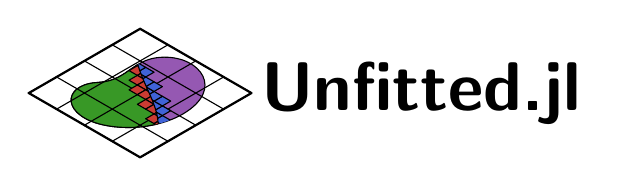
\begin{tikzpicture}[isometric view, rounded corners = 0.01mm]%
    \begin{scope}[canvas is xy plane at z = 0]
      % \fill[juliapurple] (-1cm, -1cm) rectangle (1cm, 1cm);
      \draw[\ink, thick] (-1cm, -1cm) rectangle (1cm, 1cm);


      \draw[\ink, fill = juliapurple] (-0.75, -0.3) to[closed, curve through = {(0.2, -0.7) (0.7, 0.4) (-0.15, 0.5)}] (-0.3, 0.6);
      
      \begin{scope}
        \clip (-1, -1) to[out = 10, in = 210] (1, 1) -- (-1, 1) -- cycle;
      
        \draw[\ink, fill = juliagreen] (-0.75, -0.3) to[closed, curve through = {(0.2, -0.7) (0.7, 0.4) (-0.15, 0.5)}] (-0.3, 0.6);
      \end{scope}

      \draw[\ink] (-1cm, -1cm) grid[step = 0.5cm] (1cm, 1cm);

      \begin{scope}
        \clip (-1, -1) to[out = 10, in = 210] (1, 1) -- (-1, 1) -- cycle;
        \clip (-0.75, -0.3) to[closed, curve through = {(0.2, -0.7) (0.7, 0.4) (-0.15, 0.5)}] (-0.3, 0.6);

        \draw[\ink, fill = juliared] (0.25cm, 0.3cm) rectangle ++(0.15cm, 0.15cm);
        \draw[\ink, fill = juliared] (0.25cm, 0.15cm) rectangle ++(0.15cm, 0.15cm);
        \draw[\ink, fill = juliared] (0.1cm, 0.15cm) rectangle ++(0.15cm, 0.15cm);
        \draw[\ink, fill = juliared] (0.1cm, 0cm) rectangle ++(0.15cm, 0.15cm);
        \draw[\ink, fill = juliared] (0.1cm, -0.15cm) rectangle ++(0.15cm, 0.15cm);
        \draw[\ink, fill = juliared] (-0.05cm, 0cm) rectangle ++(0.15cm, 0.15cm);
        \draw[\ink, fill = juliared] (-0.05cm, -0.15cm) rectangle ++(0.15cm, 0.15cm);
        \draw[\ink, fill = juliared] (-0.05cm, -0.3cm) rectangle ++(0.15cm, 0.15cm);
        \draw[\ink, fill = juliared] (-0.2cm, -0.3cm) rectangle ++(0.15cm, 0.15cm);
        \draw[\ink, fill = juliared] (-0.2cm, -0.45cm) rectangle ++(0.15cm, 0.15cm);
        \draw[\ink, fill = juliared] (-0.2cm, -0.6cm) rectangle ++(0.15cm, 0.15cm);
        \draw[\ink, fill = juliared] (-0.35cm, -0.6cm) rectangle ++(0.15cm, 0.15cm);
        \draw[\ink, fill = juliared] (-0.35cm, -0.75cm) rectangle ++(0.15cm, 0.15cm);
      \end{scope}

      \begin{scope}
        \clip (-1, -1) to[out = 10, in = 210] (1, 1) -- (1, -1) -- cycle;
        \clip (-0.75, -0.3) to[closed, curve through = {(0.2, -0.7) (0.7, 0.4) (-0.15, 0.5)}] (-0.3, 0.6);

        \draw[\ink, fill = juliablue] (-0.3cm, -0.7cm) rectangle ++(0.15cm, 0.15cm);
        \draw[\ink, fill = juliablue] (-0.3cm, -0.55cm) rectangle ++(0.15cm, 0.15cm);
        \draw[\ink, fill = juliablue] (-0.15cm, -0.55cm) rectangle ++(0.15cm, 0.15cm);
        \draw[\ink, fill = juliablue] (-0.15cm, -0.4cm) rectangle ++(0.15cm, 0.15cm);
        \draw[\ink, fill = juliablue] (-0cm, -0.4cm) rectangle ++(0.15cm, 0.15cm);
        \draw[\ink, fill = juliablue] (-0cm, -0.25cm) rectangle ++(0.15cm, 0.15cm);
        \draw[\ink, fill = juliablue] (-0cm, -0.1cm) rectangle ++(0.15cm, 0.15cm);
        \draw[\ink, fill = juliablue] (0.15cm, -0.1cm) rectangle ++(0.15cm, 0.15cm);
        \draw[\ink, fill = juliablue] (0.15cm, 0.05cm) rectangle ++(0.15cm, 0.15cm);
        \draw[\ink, fill = juliablue] (0.15cm, 0.2cm) rectangle ++(0.15cm, 0.15cm);
        \draw[\ink, fill = juliablue] (0.3cm, 0.2cm) rectangle ++(0.15cm, 0.15cm);
        \draw[\ink, fill = juliablue] (0.3cm, 0.35cm) rectangle ++(0.15cm, 0.15cm);
      \end{scope}

      \begin{scope}
        \clip (-0.75, -0.3) to[closed, curve through = {(0.2, -0.7) (0.7, 0.4) (-0.15, 0.5)}] (-0.3, 0.6);
        \draw[\ink] (-1, -1) to[out = 10, in = 210] (1, 1);
      \end{scope}

      \node[right, text = \ink] at (1, -1) {\Huge\sffamily\bfseries Unfitted.jl};
    \end{scope}
  \end{tikzpicture}%
\end{document}
'
%   latex -jobname=logo-dark '\def\pgfsysdriver{pgfsys-dvisvgm.def}\def\ink{white}\documentclass[margin = 1mm]{standalone}

\usepackage{tikz}
\usepackage[condensed]{roboto}

\usetikzlibrary{3d}
\usetikzlibrary{perspective}
\usetikzlibrary{hobby}

\definecolor{juliablue}{HTML}{4063D8}
\definecolor{juliagreen}{HTML}{389826}
\definecolor{juliared}{HTML}{CB3C33}
\definecolor{juliapurple}{HTML}{9558B2}

% Ink for every stroke in the drawing: the background mesh, the domain
% outline, the cell edges, the material interface and the wordmark. Fills stay
% fixed -- the four Julia colours read on either ground -- so the light and the
% dark asset differ in exactly one macro, and the dark variant is this same
% file compiled with `\ink' predefined.
%
% The README assets are SVG, built through DVI rather than PDF: dvisvgm only
% accepts PDF input via Ghostscript < 10.01 or mutool, while its DVI path is
% native and needs neither. `--no-fonts' traces the Roboto glyphs into paths
% so the wordmark does not depend on the font being installed, and `--bbox'
% restores the 1 mm margin that `--exact-bbox' would otherwise trim away.
%
%   latex -jobname=logo      '\def\pgfsysdriver{pgfsys-dvisvgm.def}\input{logo.tex}'
%   latex -jobname=logo-dark '\def\pgfsysdriver{pgfsys-dvisvgm.def}\def\ink{white}\input{logo.tex}'
%   dvisvgm --no-fonts --exact-bbox --bbox=1mm logo.dvi
%   dvisvgm --no-fonts --exact-bbox --bbox=1mm logo-dark.dvi
\providecommand{\ink}{black}

\begin{document}
  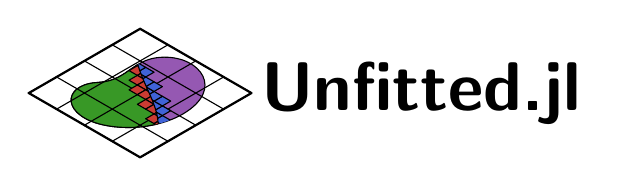
\begin{tikzpicture}[isometric view, rounded corners = 0.01mm]%
    \begin{scope}[canvas is xy plane at z = 0]
      % \fill[juliapurple] (-1cm, -1cm) rectangle (1cm, 1cm);
      \draw[\ink, thick] (-1cm, -1cm) rectangle (1cm, 1cm);


      \draw[\ink, fill = juliapurple] (-0.75, -0.3) to[closed, curve through = {(0.2, -0.7) (0.7, 0.4) (-0.15, 0.5)}] (-0.3, 0.6);
      
      \begin{scope}
        \clip (-1, -1) to[out = 10, in = 210] (1, 1) -- (-1, 1) -- cycle;
      
        \draw[\ink, fill = juliagreen] (-0.75, -0.3) to[closed, curve through = {(0.2, -0.7) (0.7, 0.4) (-0.15, 0.5)}] (-0.3, 0.6);
      \end{scope}

      \draw[\ink] (-1cm, -1cm) grid[step = 0.5cm] (1cm, 1cm);

      \begin{scope}
        \clip (-1, -1) to[out = 10, in = 210] (1, 1) -- (-1, 1) -- cycle;
        \clip (-0.75, -0.3) to[closed, curve through = {(0.2, -0.7) (0.7, 0.4) (-0.15, 0.5)}] (-0.3, 0.6);

        \draw[\ink, fill = juliared] (0.25cm, 0.3cm) rectangle ++(0.15cm, 0.15cm);
        \draw[\ink, fill = juliared] (0.25cm, 0.15cm) rectangle ++(0.15cm, 0.15cm);
        \draw[\ink, fill = juliared] (0.1cm, 0.15cm) rectangle ++(0.15cm, 0.15cm);
        \draw[\ink, fill = juliared] (0.1cm, 0cm) rectangle ++(0.15cm, 0.15cm);
        \draw[\ink, fill = juliared] (0.1cm, -0.15cm) rectangle ++(0.15cm, 0.15cm);
        \draw[\ink, fill = juliared] (-0.05cm, 0cm) rectangle ++(0.15cm, 0.15cm);
        \draw[\ink, fill = juliared] (-0.05cm, -0.15cm) rectangle ++(0.15cm, 0.15cm);
        \draw[\ink, fill = juliared] (-0.05cm, -0.3cm) rectangle ++(0.15cm, 0.15cm);
        \draw[\ink, fill = juliared] (-0.2cm, -0.3cm) rectangle ++(0.15cm, 0.15cm);
        \draw[\ink, fill = juliared] (-0.2cm, -0.45cm) rectangle ++(0.15cm, 0.15cm);
        \draw[\ink, fill = juliared] (-0.2cm, -0.6cm) rectangle ++(0.15cm, 0.15cm);
        \draw[\ink, fill = juliared] (-0.35cm, -0.6cm) rectangle ++(0.15cm, 0.15cm);
        \draw[\ink, fill = juliared] (-0.35cm, -0.75cm) rectangle ++(0.15cm, 0.15cm);
      \end{scope}

      \begin{scope}
        \clip (-1, -1) to[out = 10, in = 210] (1, 1) -- (1, -1) -- cycle;
        \clip (-0.75, -0.3) to[closed, curve through = {(0.2, -0.7) (0.7, 0.4) (-0.15, 0.5)}] (-0.3, 0.6);

        \draw[\ink, fill = juliablue] (-0.3cm, -0.7cm) rectangle ++(0.15cm, 0.15cm);
        \draw[\ink, fill = juliablue] (-0.3cm, -0.55cm) rectangle ++(0.15cm, 0.15cm);
        \draw[\ink, fill = juliablue] (-0.15cm, -0.55cm) rectangle ++(0.15cm, 0.15cm);
        \draw[\ink, fill = juliablue] (-0.15cm, -0.4cm) rectangle ++(0.15cm, 0.15cm);
        \draw[\ink, fill = juliablue] (-0cm, -0.4cm) rectangle ++(0.15cm, 0.15cm);
        \draw[\ink, fill = juliablue] (-0cm, -0.25cm) rectangle ++(0.15cm, 0.15cm);
        \draw[\ink, fill = juliablue] (-0cm, -0.1cm) rectangle ++(0.15cm, 0.15cm);
        \draw[\ink, fill = juliablue] (0.15cm, -0.1cm) rectangle ++(0.15cm, 0.15cm);
        \draw[\ink, fill = juliablue] (0.15cm, 0.05cm) rectangle ++(0.15cm, 0.15cm);
        \draw[\ink, fill = juliablue] (0.15cm, 0.2cm) rectangle ++(0.15cm, 0.15cm);
        \draw[\ink, fill = juliablue] (0.3cm, 0.2cm) rectangle ++(0.15cm, 0.15cm);
        \draw[\ink, fill = juliablue] (0.3cm, 0.35cm) rectangle ++(0.15cm, 0.15cm);
      \end{scope}

      \begin{scope}
        \clip (-0.75, -0.3) to[closed, curve through = {(0.2, -0.7) (0.7, 0.4) (-0.15, 0.5)}] (-0.3, 0.6);
        \draw[\ink] (-1, -1) to[out = 10, in = 210] (1, 1);
      \end{scope}

      \node[right, text = \ink] at (1, -1) {\Huge\sffamily\bfseries Unfitted.jl};
    \end{scope}
  \end{tikzpicture}%
\end{document}
'
%   dvisvgm --no-fonts --exact-bbox --bbox=1mm logo.dvi
%   dvisvgm --no-fonts --exact-bbox --bbox=1mm logo-dark.dvi
\providecommand{\ink}{black}

\begin{document}
  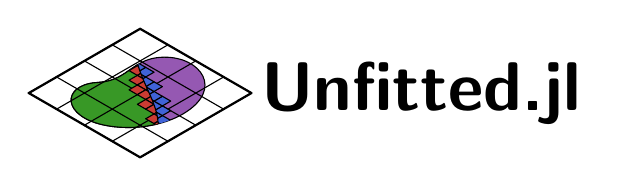
\begin{tikzpicture}[isometric view, rounded corners = 0.01mm]%
    \begin{scope}[canvas is xy plane at z = 0]
      % \fill[juliapurple] (-1cm, -1cm) rectangle (1cm, 1cm);
      \draw[\ink, thick] (-1cm, -1cm) rectangle (1cm, 1cm);


      \draw[\ink, fill = juliapurple] (-0.75, -0.3) to[closed, curve through = {(0.2, -0.7) (0.7, 0.4) (-0.15, 0.5)}] (-0.3, 0.6);
      
      \begin{scope}
        \clip (-1, -1) to[out = 10, in = 210] (1, 1) -- (-1, 1) -- cycle;
      
        \draw[\ink, fill = juliagreen] (-0.75, -0.3) to[closed, curve through = {(0.2, -0.7) (0.7, 0.4) (-0.15, 0.5)}] (-0.3, 0.6);
      \end{scope}

      \draw[\ink] (-1cm, -1cm) grid[step = 0.5cm] (1cm, 1cm);

      \begin{scope}
        \clip (-1, -1) to[out = 10, in = 210] (1, 1) -- (-1, 1) -- cycle;
        \clip (-0.75, -0.3) to[closed, curve through = {(0.2, -0.7) (0.7, 0.4) (-0.15, 0.5)}] (-0.3, 0.6);

        \draw[\ink, fill = juliared] (0.25cm, 0.3cm) rectangle ++(0.15cm, 0.15cm);
        \draw[\ink, fill = juliared] (0.25cm, 0.15cm) rectangle ++(0.15cm, 0.15cm);
        \draw[\ink, fill = juliared] (0.1cm, 0.15cm) rectangle ++(0.15cm, 0.15cm);
        \draw[\ink, fill = juliared] (0.1cm, 0cm) rectangle ++(0.15cm, 0.15cm);
        \draw[\ink, fill = juliared] (0.1cm, -0.15cm) rectangle ++(0.15cm, 0.15cm);
        \draw[\ink, fill = juliared] (-0.05cm, 0cm) rectangle ++(0.15cm, 0.15cm);
        \draw[\ink, fill = juliared] (-0.05cm, -0.15cm) rectangle ++(0.15cm, 0.15cm);
        \draw[\ink, fill = juliared] (-0.05cm, -0.3cm) rectangle ++(0.15cm, 0.15cm);
        \draw[\ink, fill = juliared] (-0.2cm, -0.3cm) rectangle ++(0.15cm, 0.15cm);
        \draw[\ink, fill = juliared] (-0.2cm, -0.45cm) rectangle ++(0.15cm, 0.15cm);
        \draw[\ink, fill = juliared] (-0.2cm, -0.6cm) rectangle ++(0.15cm, 0.15cm);
        \draw[\ink, fill = juliared] (-0.35cm, -0.6cm) rectangle ++(0.15cm, 0.15cm);
        \draw[\ink, fill = juliared] (-0.35cm, -0.75cm) rectangle ++(0.15cm, 0.15cm);
      \end{scope}

      \begin{scope}
        \clip (-1, -1) to[out = 10, in = 210] (1, 1) -- (1, -1) -- cycle;
        \clip (-0.75, -0.3) to[closed, curve through = {(0.2, -0.7) (0.7, 0.4) (-0.15, 0.5)}] (-0.3, 0.6);

        \draw[\ink, fill = juliablue] (-0.3cm, -0.7cm) rectangle ++(0.15cm, 0.15cm);
        \draw[\ink, fill = juliablue] (-0.3cm, -0.55cm) rectangle ++(0.15cm, 0.15cm);
        \draw[\ink, fill = juliablue] (-0.15cm, -0.55cm) rectangle ++(0.15cm, 0.15cm);
        \draw[\ink, fill = juliablue] (-0.15cm, -0.4cm) rectangle ++(0.15cm, 0.15cm);
        \draw[\ink, fill = juliablue] (-0cm, -0.4cm) rectangle ++(0.15cm, 0.15cm);
        \draw[\ink, fill = juliablue] (-0cm, -0.25cm) rectangle ++(0.15cm, 0.15cm);
        \draw[\ink, fill = juliablue] (-0cm, -0.1cm) rectangle ++(0.15cm, 0.15cm);
        \draw[\ink, fill = juliablue] (0.15cm, -0.1cm) rectangle ++(0.15cm, 0.15cm);
        \draw[\ink, fill = juliablue] (0.15cm, 0.05cm) rectangle ++(0.15cm, 0.15cm);
        \draw[\ink, fill = juliablue] (0.15cm, 0.2cm) rectangle ++(0.15cm, 0.15cm);
        \draw[\ink, fill = juliablue] (0.3cm, 0.2cm) rectangle ++(0.15cm, 0.15cm);
        \draw[\ink, fill = juliablue] (0.3cm, 0.35cm) rectangle ++(0.15cm, 0.15cm);
      \end{scope}

      \begin{scope}
        \clip (-0.75, -0.3) to[closed, curve through = {(0.2, -0.7) (0.7, 0.4) (-0.15, 0.5)}] (-0.3, 0.6);
        \draw[\ink] (-1, -1) to[out = 10, in = 210] (1, 1);
      \end{scope}

      \node[right, text = \ink] at (1, -1) {\Huge\sffamily\bfseries Unfitted.jl};
    \end{scope}
  \end{tikzpicture}%
\end{document}
'
%   latex -jobname=logo-dark '\def\pgfsysdriver{pgfsys-dvisvgm.def}\def\ink{white}\documentclass[margin = 1mm]{standalone}

\usepackage{tikz}
\usepackage[condensed]{roboto}

\usetikzlibrary{3d}
\usetikzlibrary{perspective}
\usetikzlibrary{hobby}

\definecolor{juliablue}{HTML}{4063D8}
\definecolor{juliagreen}{HTML}{389826}
\definecolor{juliared}{HTML}{CB3C33}
\definecolor{juliapurple}{HTML}{9558B2}

% Ink for every stroke in the drawing: the background mesh, the domain
% outline, the cell edges, the material interface and the wordmark. Fills stay
% fixed -- the four Julia colours read on either ground -- so the light and the
% dark asset differ in exactly one macro, and the dark variant is this same
% file compiled with `\ink' predefined.
%
% The README assets are SVG, built through DVI rather than PDF: dvisvgm only
% accepts PDF input via Ghostscript < 10.01 or mutool, while its DVI path is
% native and needs neither. `--no-fonts' traces the Roboto glyphs into paths
% so the wordmark does not depend on the font being installed, and `--bbox'
% restores the 1 mm margin that `--exact-bbox' would otherwise trim away.
%
%   latex -jobname=logo      '\def\pgfsysdriver{pgfsys-dvisvgm.def}\documentclass[margin = 1mm]{standalone}

\usepackage{tikz}
\usepackage[condensed]{roboto}

\usetikzlibrary{3d}
\usetikzlibrary{perspective}
\usetikzlibrary{hobby}

\definecolor{juliablue}{HTML}{4063D8}
\definecolor{juliagreen}{HTML}{389826}
\definecolor{juliared}{HTML}{CB3C33}
\definecolor{juliapurple}{HTML}{9558B2}

% Ink for every stroke in the drawing: the background mesh, the domain
% outline, the cell edges, the material interface and the wordmark. Fills stay
% fixed -- the four Julia colours read on either ground -- so the light and the
% dark asset differ in exactly one macro, and the dark variant is this same
% file compiled with `\ink' predefined.
%
% The README assets are SVG, built through DVI rather than PDF: dvisvgm only
% accepts PDF input via Ghostscript < 10.01 or mutool, while its DVI path is
% native and needs neither. `--no-fonts' traces the Roboto glyphs into paths
% so the wordmark does not depend on the font being installed, and `--bbox'
% restores the 1 mm margin that `--exact-bbox' would otherwise trim away.
%
%   latex -jobname=logo      '\def\pgfsysdriver{pgfsys-dvisvgm.def}\input{logo.tex}'
%   latex -jobname=logo-dark '\def\pgfsysdriver{pgfsys-dvisvgm.def}\def\ink{white}\input{logo.tex}'
%   dvisvgm --no-fonts --exact-bbox --bbox=1mm logo.dvi
%   dvisvgm --no-fonts --exact-bbox --bbox=1mm logo-dark.dvi
\providecommand{\ink}{black}

\begin{document}
  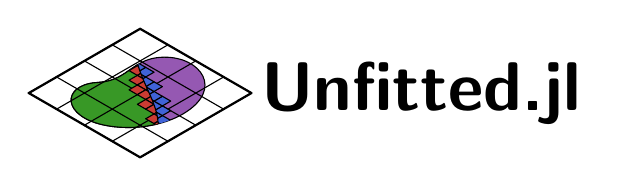
\begin{tikzpicture}[isometric view, rounded corners = 0.01mm]%
    \begin{scope}[canvas is xy plane at z = 0]
      % \fill[juliapurple] (-1cm, -1cm) rectangle (1cm, 1cm);
      \draw[\ink, thick] (-1cm, -1cm) rectangle (1cm, 1cm);


      \draw[\ink, fill = juliapurple] (-0.75, -0.3) to[closed, curve through = {(0.2, -0.7) (0.7, 0.4) (-0.15, 0.5)}] (-0.3, 0.6);
      
      \begin{scope}
        \clip (-1, -1) to[out = 10, in = 210] (1, 1) -- (-1, 1) -- cycle;
      
        \draw[\ink, fill = juliagreen] (-0.75, -0.3) to[closed, curve through = {(0.2, -0.7) (0.7, 0.4) (-0.15, 0.5)}] (-0.3, 0.6);
      \end{scope}

      \draw[\ink] (-1cm, -1cm) grid[step = 0.5cm] (1cm, 1cm);

      \begin{scope}
        \clip (-1, -1) to[out = 10, in = 210] (1, 1) -- (-1, 1) -- cycle;
        \clip (-0.75, -0.3) to[closed, curve through = {(0.2, -0.7) (0.7, 0.4) (-0.15, 0.5)}] (-0.3, 0.6);

        \draw[\ink, fill = juliared] (0.25cm, 0.3cm) rectangle ++(0.15cm, 0.15cm);
        \draw[\ink, fill = juliared] (0.25cm, 0.15cm) rectangle ++(0.15cm, 0.15cm);
        \draw[\ink, fill = juliared] (0.1cm, 0.15cm) rectangle ++(0.15cm, 0.15cm);
        \draw[\ink, fill = juliared] (0.1cm, 0cm) rectangle ++(0.15cm, 0.15cm);
        \draw[\ink, fill = juliared] (0.1cm, -0.15cm) rectangle ++(0.15cm, 0.15cm);
        \draw[\ink, fill = juliared] (-0.05cm, 0cm) rectangle ++(0.15cm, 0.15cm);
        \draw[\ink, fill = juliared] (-0.05cm, -0.15cm) rectangle ++(0.15cm, 0.15cm);
        \draw[\ink, fill = juliared] (-0.05cm, -0.3cm) rectangle ++(0.15cm, 0.15cm);
        \draw[\ink, fill = juliared] (-0.2cm, -0.3cm) rectangle ++(0.15cm, 0.15cm);
        \draw[\ink, fill = juliared] (-0.2cm, -0.45cm) rectangle ++(0.15cm, 0.15cm);
        \draw[\ink, fill = juliared] (-0.2cm, -0.6cm) rectangle ++(0.15cm, 0.15cm);
        \draw[\ink, fill = juliared] (-0.35cm, -0.6cm) rectangle ++(0.15cm, 0.15cm);
        \draw[\ink, fill = juliared] (-0.35cm, -0.75cm) rectangle ++(0.15cm, 0.15cm);
      \end{scope}

      \begin{scope}
        \clip (-1, -1) to[out = 10, in = 210] (1, 1) -- (1, -1) -- cycle;
        \clip (-0.75, -0.3) to[closed, curve through = {(0.2, -0.7) (0.7, 0.4) (-0.15, 0.5)}] (-0.3, 0.6);

        \draw[\ink, fill = juliablue] (-0.3cm, -0.7cm) rectangle ++(0.15cm, 0.15cm);
        \draw[\ink, fill = juliablue] (-0.3cm, -0.55cm) rectangle ++(0.15cm, 0.15cm);
        \draw[\ink, fill = juliablue] (-0.15cm, -0.55cm) rectangle ++(0.15cm, 0.15cm);
        \draw[\ink, fill = juliablue] (-0.15cm, -0.4cm) rectangle ++(0.15cm, 0.15cm);
        \draw[\ink, fill = juliablue] (-0cm, -0.4cm) rectangle ++(0.15cm, 0.15cm);
        \draw[\ink, fill = juliablue] (-0cm, -0.25cm) rectangle ++(0.15cm, 0.15cm);
        \draw[\ink, fill = juliablue] (-0cm, -0.1cm) rectangle ++(0.15cm, 0.15cm);
        \draw[\ink, fill = juliablue] (0.15cm, -0.1cm) rectangle ++(0.15cm, 0.15cm);
        \draw[\ink, fill = juliablue] (0.15cm, 0.05cm) rectangle ++(0.15cm, 0.15cm);
        \draw[\ink, fill = juliablue] (0.15cm, 0.2cm) rectangle ++(0.15cm, 0.15cm);
        \draw[\ink, fill = juliablue] (0.3cm, 0.2cm) rectangle ++(0.15cm, 0.15cm);
        \draw[\ink, fill = juliablue] (0.3cm, 0.35cm) rectangle ++(0.15cm, 0.15cm);
      \end{scope}

      \begin{scope}
        \clip (-0.75, -0.3) to[closed, curve through = {(0.2, -0.7) (0.7, 0.4) (-0.15, 0.5)}] (-0.3, 0.6);
        \draw[\ink] (-1, -1) to[out = 10, in = 210] (1, 1);
      \end{scope}

      \node[right, text = \ink] at (1, -1) {\Huge\sffamily\bfseries Unfitted.jl};
    \end{scope}
  \end{tikzpicture}%
\end{document}
'
%   latex -jobname=logo-dark '\def\pgfsysdriver{pgfsys-dvisvgm.def}\def\ink{white}\documentclass[margin = 1mm]{standalone}

\usepackage{tikz}
\usepackage[condensed]{roboto}

\usetikzlibrary{3d}
\usetikzlibrary{perspective}
\usetikzlibrary{hobby}

\definecolor{juliablue}{HTML}{4063D8}
\definecolor{juliagreen}{HTML}{389826}
\definecolor{juliared}{HTML}{CB3C33}
\definecolor{juliapurple}{HTML}{9558B2}

% Ink for every stroke in the drawing: the background mesh, the domain
% outline, the cell edges, the material interface and the wordmark. Fills stay
% fixed -- the four Julia colours read on either ground -- so the light and the
% dark asset differ in exactly one macro, and the dark variant is this same
% file compiled with `\ink' predefined.
%
% The README assets are SVG, built through DVI rather than PDF: dvisvgm only
% accepts PDF input via Ghostscript < 10.01 or mutool, while its DVI path is
% native and needs neither. `--no-fonts' traces the Roboto glyphs into paths
% so the wordmark does not depend on the font being installed, and `--bbox'
% restores the 1 mm margin that `--exact-bbox' would otherwise trim away.
%
%   latex -jobname=logo      '\def\pgfsysdriver{pgfsys-dvisvgm.def}\input{logo.tex}'
%   latex -jobname=logo-dark '\def\pgfsysdriver{pgfsys-dvisvgm.def}\def\ink{white}\input{logo.tex}'
%   dvisvgm --no-fonts --exact-bbox --bbox=1mm logo.dvi
%   dvisvgm --no-fonts --exact-bbox --bbox=1mm logo-dark.dvi
\providecommand{\ink}{black}

\begin{document}
  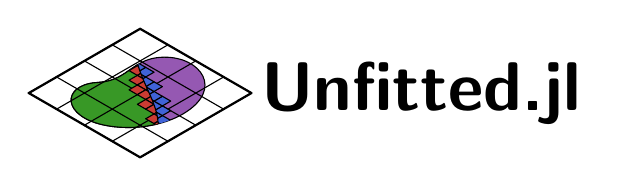
\begin{tikzpicture}[isometric view, rounded corners = 0.01mm]%
    \begin{scope}[canvas is xy plane at z = 0]
      % \fill[juliapurple] (-1cm, -1cm) rectangle (1cm, 1cm);
      \draw[\ink, thick] (-1cm, -1cm) rectangle (1cm, 1cm);


      \draw[\ink, fill = juliapurple] (-0.75, -0.3) to[closed, curve through = {(0.2, -0.7) (0.7, 0.4) (-0.15, 0.5)}] (-0.3, 0.6);
      
      \begin{scope}
        \clip (-1, -1) to[out = 10, in = 210] (1, 1) -- (-1, 1) -- cycle;
      
        \draw[\ink, fill = juliagreen] (-0.75, -0.3) to[closed, curve through = {(0.2, -0.7) (0.7, 0.4) (-0.15, 0.5)}] (-0.3, 0.6);
      \end{scope}

      \draw[\ink] (-1cm, -1cm) grid[step = 0.5cm] (1cm, 1cm);

      \begin{scope}
        \clip (-1, -1) to[out = 10, in = 210] (1, 1) -- (-1, 1) -- cycle;
        \clip (-0.75, -0.3) to[closed, curve through = {(0.2, -0.7) (0.7, 0.4) (-0.15, 0.5)}] (-0.3, 0.6);

        \draw[\ink, fill = juliared] (0.25cm, 0.3cm) rectangle ++(0.15cm, 0.15cm);
        \draw[\ink, fill = juliared] (0.25cm, 0.15cm) rectangle ++(0.15cm, 0.15cm);
        \draw[\ink, fill = juliared] (0.1cm, 0.15cm) rectangle ++(0.15cm, 0.15cm);
        \draw[\ink, fill = juliared] (0.1cm, 0cm) rectangle ++(0.15cm, 0.15cm);
        \draw[\ink, fill = juliared] (0.1cm, -0.15cm) rectangle ++(0.15cm, 0.15cm);
        \draw[\ink, fill = juliared] (-0.05cm, 0cm) rectangle ++(0.15cm, 0.15cm);
        \draw[\ink, fill = juliared] (-0.05cm, -0.15cm) rectangle ++(0.15cm, 0.15cm);
        \draw[\ink, fill = juliared] (-0.05cm, -0.3cm) rectangle ++(0.15cm, 0.15cm);
        \draw[\ink, fill = juliared] (-0.2cm, -0.3cm) rectangle ++(0.15cm, 0.15cm);
        \draw[\ink, fill = juliared] (-0.2cm, -0.45cm) rectangle ++(0.15cm, 0.15cm);
        \draw[\ink, fill = juliared] (-0.2cm, -0.6cm) rectangle ++(0.15cm, 0.15cm);
        \draw[\ink, fill = juliared] (-0.35cm, -0.6cm) rectangle ++(0.15cm, 0.15cm);
        \draw[\ink, fill = juliared] (-0.35cm, -0.75cm) rectangle ++(0.15cm, 0.15cm);
      \end{scope}

      \begin{scope}
        \clip (-1, -1) to[out = 10, in = 210] (1, 1) -- (1, -1) -- cycle;
        \clip (-0.75, -0.3) to[closed, curve through = {(0.2, -0.7) (0.7, 0.4) (-0.15, 0.5)}] (-0.3, 0.6);

        \draw[\ink, fill = juliablue] (-0.3cm, -0.7cm) rectangle ++(0.15cm, 0.15cm);
        \draw[\ink, fill = juliablue] (-0.3cm, -0.55cm) rectangle ++(0.15cm, 0.15cm);
        \draw[\ink, fill = juliablue] (-0.15cm, -0.55cm) rectangle ++(0.15cm, 0.15cm);
        \draw[\ink, fill = juliablue] (-0.15cm, -0.4cm) rectangle ++(0.15cm, 0.15cm);
        \draw[\ink, fill = juliablue] (-0cm, -0.4cm) rectangle ++(0.15cm, 0.15cm);
        \draw[\ink, fill = juliablue] (-0cm, -0.25cm) rectangle ++(0.15cm, 0.15cm);
        \draw[\ink, fill = juliablue] (-0cm, -0.1cm) rectangle ++(0.15cm, 0.15cm);
        \draw[\ink, fill = juliablue] (0.15cm, -0.1cm) rectangle ++(0.15cm, 0.15cm);
        \draw[\ink, fill = juliablue] (0.15cm, 0.05cm) rectangle ++(0.15cm, 0.15cm);
        \draw[\ink, fill = juliablue] (0.15cm, 0.2cm) rectangle ++(0.15cm, 0.15cm);
        \draw[\ink, fill = juliablue] (0.3cm, 0.2cm) rectangle ++(0.15cm, 0.15cm);
        \draw[\ink, fill = juliablue] (0.3cm, 0.35cm) rectangle ++(0.15cm, 0.15cm);
      \end{scope}

      \begin{scope}
        \clip (-0.75, -0.3) to[closed, curve through = {(0.2, -0.7) (0.7, 0.4) (-0.15, 0.5)}] (-0.3, 0.6);
        \draw[\ink] (-1, -1) to[out = 10, in = 210] (1, 1);
      \end{scope}

      \node[right, text = \ink] at (1, -1) {\Huge\sffamily\bfseries Unfitted.jl};
    \end{scope}
  \end{tikzpicture}%
\end{document}
'
%   dvisvgm --no-fonts --exact-bbox --bbox=1mm logo.dvi
%   dvisvgm --no-fonts --exact-bbox --bbox=1mm logo-dark.dvi
\providecommand{\ink}{black}

\begin{document}
  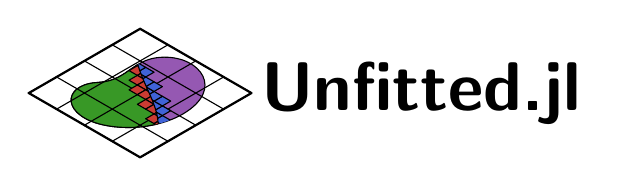
\begin{tikzpicture}[isometric view, rounded corners = 0.01mm]%
    \begin{scope}[canvas is xy plane at z = 0]
      % \fill[juliapurple] (-1cm, -1cm) rectangle (1cm, 1cm);
      \draw[\ink, thick] (-1cm, -1cm) rectangle (1cm, 1cm);


      \draw[\ink, fill = juliapurple] (-0.75, -0.3) to[closed, curve through = {(0.2, -0.7) (0.7, 0.4) (-0.15, 0.5)}] (-0.3, 0.6);
      
      \begin{scope}
        \clip (-1, -1) to[out = 10, in = 210] (1, 1) -- (-1, 1) -- cycle;
      
        \draw[\ink, fill = juliagreen] (-0.75, -0.3) to[closed, curve through = {(0.2, -0.7) (0.7, 0.4) (-0.15, 0.5)}] (-0.3, 0.6);
      \end{scope}

      \draw[\ink] (-1cm, -1cm) grid[step = 0.5cm] (1cm, 1cm);

      \begin{scope}
        \clip (-1, -1) to[out = 10, in = 210] (1, 1) -- (-1, 1) -- cycle;
        \clip (-0.75, -0.3) to[closed, curve through = {(0.2, -0.7) (0.7, 0.4) (-0.15, 0.5)}] (-0.3, 0.6);

        \draw[\ink, fill = juliared] (0.25cm, 0.3cm) rectangle ++(0.15cm, 0.15cm);
        \draw[\ink, fill = juliared] (0.25cm, 0.15cm) rectangle ++(0.15cm, 0.15cm);
        \draw[\ink, fill = juliared] (0.1cm, 0.15cm) rectangle ++(0.15cm, 0.15cm);
        \draw[\ink, fill = juliared] (0.1cm, 0cm) rectangle ++(0.15cm, 0.15cm);
        \draw[\ink, fill = juliared] (0.1cm, -0.15cm) rectangle ++(0.15cm, 0.15cm);
        \draw[\ink, fill = juliared] (-0.05cm, 0cm) rectangle ++(0.15cm, 0.15cm);
        \draw[\ink, fill = juliared] (-0.05cm, -0.15cm) rectangle ++(0.15cm, 0.15cm);
        \draw[\ink, fill = juliared] (-0.05cm, -0.3cm) rectangle ++(0.15cm, 0.15cm);
        \draw[\ink, fill = juliared] (-0.2cm, -0.3cm) rectangle ++(0.15cm, 0.15cm);
        \draw[\ink, fill = juliared] (-0.2cm, -0.45cm) rectangle ++(0.15cm, 0.15cm);
        \draw[\ink, fill = juliared] (-0.2cm, -0.6cm) rectangle ++(0.15cm, 0.15cm);
        \draw[\ink, fill = juliared] (-0.35cm, -0.6cm) rectangle ++(0.15cm, 0.15cm);
        \draw[\ink, fill = juliared] (-0.35cm, -0.75cm) rectangle ++(0.15cm, 0.15cm);
      \end{scope}

      \begin{scope}
        \clip (-1, -1) to[out = 10, in = 210] (1, 1) -- (1, -1) -- cycle;
        \clip (-0.75, -0.3) to[closed, curve through = {(0.2, -0.7) (0.7, 0.4) (-0.15, 0.5)}] (-0.3, 0.6);

        \draw[\ink, fill = juliablue] (-0.3cm, -0.7cm) rectangle ++(0.15cm, 0.15cm);
        \draw[\ink, fill = juliablue] (-0.3cm, -0.55cm) rectangle ++(0.15cm, 0.15cm);
        \draw[\ink, fill = juliablue] (-0.15cm, -0.55cm) rectangle ++(0.15cm, 0.15cm);
        \draw[\ink, fill = juliablue] (-0.15cm, -0.4cm) rectangle ++(0.15cm, 0.15cm);
        \draw[\ink, fill = juliablue] (-0cm, -0.4cm) rectangle ++(0.15cm, 0.15cm);
        \draw[\ink, fill = juliablue] (-0cm, -0.25cm) rectangle ++(0.15cm, 0.15cm);
        \draw[\ink, fill = juliablue] (-0cm, -0.1cm) rectangle ++(0.15cm, 0.15cm);
        \draw[\ink, fill = juliablue] (0.15cm, -0.1cm) rectangle ++(0.15cm, 0.15cm);
        \draw[\ink, fill = juliablue] (0.15cm, 0.05cm) rectangle ++(0.15cm, 0.15cm);
        \draw[\ink, fill = juliablue] (0.15cm, 0.2cm) rectangle ++(0.15cm, 0.15cm);
        \draw[\ink, fill = juliablue] (0.3cm, 0.2cm) rectangle ++(0.15cm, 0.15cm);
        \draw[\ink, fill = juliablue] (0.3cm, 0.35cm) rectangle ++(0.15cm, 0.15cm);
      \end{scope}

      \begin{scope}
        \clip (-0.75, -0.3) to[closed, curve through = {(0.2, -0.7) (0.7, 0.4) (-0.15, 0.5)}] (-0.3, 0.6);
        \draw[\ink] (-1, -1) to[out = 10, in = 210] (1, 1);
      \end{scope}

      \node[right, text = \ink] at (1, -1) {\Huge\sffamily\bfseries Unfitted.jl};
    \end{scope}
  \end{tikzpicture}%
\end{document}
'
%   dvisvgm --no-fonts --exact-bbox --bbox=1mm logo.dvi
%   dvisvgm --no-fonts --exact-bbox --bbox=1mm logo-dark.dvi
\providecommand{\ink}{black}

\begin{document}
  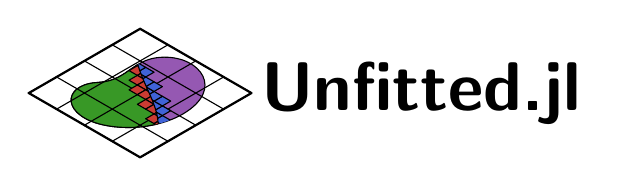
\begin{tikzpicture}[isometric view, rounded corners = 0.01mm]%
    \begin{scope}[canvas is xy plane at z = 0]
      % \fill[juliapurple] (-1cm, -1cm) rectangle (1cm, 1cm);
      \draw[\ink, thick] (-1cm, -1cm) rectangle (1cm, 1cm);


      \draw[\ink, fill = juliapurple] (-0.75, -0.3) to[closed, curve through = {(0.2, -0.7) (0.7, 0.4) (-0.15, 0.5)}] (-0.3, 0.6);
      
      \begin{scope}
        \clip (-1, -1) to[out = 10, in = 210] (1, 1) -- (-1, 1) -- cycle;
      
        \draw[\ink, fill = juliagreen] (-0.75, -0.3) to[closed, curve through = {(0.2, -0.7) (0.7, 0.4) (-0.15, 0.5)}] (-0.3, 0.6);
      \end{scope}

      \draw[\ink] (-1cm, -1cm) grid[step = 0.5cm] (1cm, 1cm);

      \begin{scope}
        \clip (-1, -1) to[out = 10, in = 210] (1, 1) -- (-1, 1) -- cycle;
        \clip (-0.75, -0.3) to[closed, curve through = {(0.2, -0.7) (0.7, 0.4) (-0.15, 0.5)}] (-0.3, 0.6);

        \draw[\ink, fill = juliared] (0.25cm, 0.3cm) rectangle ++(0.15cm, 0.15cm);
        \draw[\ink, fill = juliared] (0.25cm, 0.15cm) rectangle ++(0.15cm, 0.15cm);
        \draw[\ink, fill = juliared] (0.1cm, 0.15cm) rectangle ++(0.15cm, 0.15cm);
        \draw[\ink, fill = juliared] (0.1cm, 0cm) rectangle ++(0.15cm, 0.15cm);
        \draw[\ink, fill = juliared] (0.1cm, -0.15cm) rectangle ++(0.15cm, 0.15cm);
        \draw[\ink, fill = juliared] (-0.05cm, 0cm) rectangle ++(0.15cm, 0.15cm);
        \draw[\ink, fill = juliared] (-0.05cm, -0.15cm) rectangle ++(0.15cm, 0.15cm);
        \draw[\ink, fill = juliared] (-0.05cm, -0.3cm) rectangle ++(0.15cm, 0.15cm);
        \draw[\ink, fill = juliared] (-0.2cm, -0.3cm) rectangle ++(0.15cm, 0.15cm);
        \draw[\ink, fill = juliared] (-0.2cm, -0.45cm) rectangle ++(0.15cm, 0.15cm);
        \draw[\ink, fill = juliared] (-0.2cm, -0.6cm) rectangle ++(0.15cm, 0.15cm);
        \draw[\ink, fill = juliared] (-0.35cm, -0.6cm) rectangle ++(0.15cm, 0.15cm);
        \draw[\ink, fill = juliared] (-0.35cm, -0.75cm) rectangle ++(0.15cm, 0.15cm);
      \end{scope}

      \begin{scope}
        \clip (-1, -1) to[out = 10, in = 210] (1, 1) -- (1, -1) -- cycle;
        \clip (-0.75, -0.3) to[closed, curve through = {(0.2, -0.7) (0.7, 0.4) (-0.15, 0.5)}] (-0.3, 0.6);

        \draw[\ink, fill = juliablue] (-0.3cm, -0.7cm) rectangle ++(0.15cm, 0.15cm);
        \draw[\ink, fill = juliablue] (-0.3cm, -0.55cm) rectangle ++(0.15cm, 0.15cm);
        \draw[\ink, fill = juliablue] (-0.15cm, -0.55cm) rectangle ++(0.15cm, 0.15cm);
        \draw[\ink, fill = juliablue] (-0.15cm, -0.4cm) rectangle ++(0.15cm, 0.15cm);
        \draw[\ink, fill = juliablue] (-0cm, -0.4cm) rectangle ++(0.15cm, 0.15cm);
        \draw[\ink, fill = juliablue] (-0cm, -0.25cm) rectangle ++(0.15cm, 0.15cm);
        \draw[\ink, fill = juliablue] (-0cm, -0.1cm) rectangle ++(0.15cm, 0.15cm);
        \draw[\ink, fill = juliablue] (0.15cm, -0.1cm) rectangle ++(0.15cm, 0.15cm);
        \draw[\ink, fill = juliablue] (0.15cm, 0.05cm) rectangle ++(0.15cm, 0.15cm);
        \draw[\ink, fill = juliablue] (0.15cm, 0.2cm) rectangle ++(0.15cm, 0.15cm);
        \draw[\ink, fill = juliablue] (0.3cm, 0.2cm) rectangle ++(0.15cm, 0.15cm);
        \draw[\ink, fill = juliablue] (0.3cm, 0.35cm) rectangle ++(0.15cm, 0.15cm);
      \end{scope}

      \begin{scope}
        \clip (-0.75, -0.3) to[closed, curve through = {(0.2, -0.7) (0.7, 0.4) (-0.15, 0.5)}] (-0.3, 0.6);
        \draw[\ink] (-1, -1) to[out = 10, in = 210] (1, 1);
      \end{scope}

      \node[right, text = \ink] at (1, -1) {\Huge\sffamily\bfseries Unfitted.jl};
    \end{scope}
  \end{tikzpicture}%
\end{document}
'
%   latex -jobname=logo-dark '\def\pgfsysdriver{pgfsys-dvisvgm.def}\def\ink{white}\documentclass[margin = 1mm]{standalone}

\usepackage{tikz}
\usepackage[condensed]{roboto}

\usetikzlibrary{3d}
\usetikzlibrary{perspective}
\usetikzlibrary{hobby}

\definecolor{juliablue}{HTML}{4063D8}
\definecolor{juliagreen}{HTML}{389826}
\definecolor{juliared}{HTML}{CB3C33}
\definecolor{juliapurple}{HTML}{9558B2}

% Ink for every stroke in the drawing: the background mesh, the domain
% outline, the cell edges, the material interface and the wordmark. Fills stay
% fixed -- the four Julia colours read on either ground -- so the light and the
% dark asset differ in exactly one macro, and the dark variant is this same
% file compiled with `\ink' predefined.
%
% The README assets are SVG, built through DVI rather than PDF: dvisvgm only
% accepts PDF input via Ghostscript < 10.01 or mutool, while its DVI path is
% native and needs neither. `--no-fonts' traces the Roboto glyphs into paths
% so the wordmark does not depend on the font being installed, and `--bbox'
% restores the 1 mm margin that `--exact-bbox' would otherwise trim away.
%
%   latex -jobname=logo      '\def\pgfsysdriver{pgfsys-dvisvgm.def}\documentclass[margin = 1mm]{standalone}

\usepackage{tikz}
\usepackage[condensed]{roboto}

\usetikzlibrary{3d}
\usetikzlibrary{perspective}
\usetikzlibrary{hobby}

\definecolor{juliablue}{HTML}{4063D8}
\definecolor{juliagreen}{HTML}{389826}
\definecolor{juliared}{HTML}{CB3C33}
\definecolor{juliapurple}{HTML}{9558B2}

% Ink for every stroke in the drawing: the background mesh, the domain
% outline, the cell edges, the material interface and the wordmark. Fills stay
% fixed -- the four Julia colours read on either ground -- so the light and the
% dark asset differ in exactly one macro, and the dark variant is this same
% file compiled with `\ink' predefined.
%
% The README assets are SVG, built through DVI rather than PDF: dvisvgm only
% accepts PDF input via Ghostscript < 10.01 or mutool, while its DVI path is
% native and needs neither. `--no-fonts' traces the Roboto glyphs into paths
% so the wordmark does not depend on the font being installed, and `--bbox'
% restores the 1 mm margin that `--exact-bbox' would otherwise trim away.
%
%   latex -jobname=logo      '\def\pgfsysdriver{pgfsys-dvisvgm.def}\documentclass[margin = 1mm]{standalone}

\usepackage{tikz}
\usepackage[condensed]{roboto}

\usetikzlibrary{3d}
\usetikzlibrary{perspective}
\usetikzlibrary{hobby}

\definecolor{juliablue}{HTML}{4063D8}
\definecolor{juliagreen}{HTML}{389826}
\definecolor{juliared}{HTML}{CB3C33}
\definecolor{juliapurple}{HTML}{9558B2}

% Ink for every stroke in the drawing: the background mesh, the domain
% outline, the cell edges, the material interface and the wordmark. Fills stay
% fixed -- the four Julia colours read on either ground -- so the light and the
% dark asset differ in exactly one macro, and the dark variant is this same
% file compiled with `\ink' predefined.
%
% The README assets are SVG, built through DVI rather than PDF: dvisvgm only
% accepts PDF input via Ghostscript < 10.01 or mutool, while its DVI path is
% native and needs neither. `--no-fonts' traces the Roboto glyphs into paths
% so the wordmark does not depend on the font being installed, and `--bbox'
% restores the 1 mm margin that `--exact-bbox' would otherwise trim away.
%
%   latex -jobname=logo      '\def\pgfsysdriver{pgfsys-dvisvgm.def}\input{logo.tex}'
%   latex -jobname=logo-dark '\def\pgfsysdriver{pgfsys-dvisvgm.def}\def\ink{white}\input{logo.tex}'
%   dvisvgm --no-fonts --exact-bbox --bbox=1mm logo.dvi
%   dvisvgm --no-fonts --exact-bbox --bbox=1mm logo-dark.dvi
\providecommand{\ink}{black}

\begin{document}
  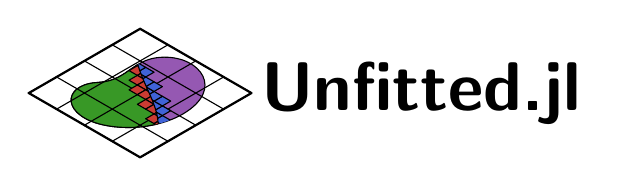
\begin{tikzpicture}[isometric view, rounded corners = 0.01mm]%
    \begin{scope}[canvas is xy plane at z = 0]
      % \fill[juliapurple] (-1cm, -1cm) rectangle (1cm, 1cm);
      \draw[\ink, thick] (-1cm, -1cm) rectangle (1cm, 1cm);


      \draw[\ink, fill = juliapurple] (-0.75, -0.3) to[closed, curve through = {(0.2, -0.7) (0.7, 0.4) (-0.15, 0.5)}] (-0.3, 0.6);
      
      \begin{scope}
        \clip (-1, -1) to[out = 10, in = 210] (1, 1) -- (-1, 1) -- cycle;
      
        \draw[\ink, fill = juliagreen] (-0.75, -0.3) to[closed, curve through = {(0.2, -0.7) (0.7, 0.4) (-0.15, 0.5)}] (-0.3, 0.6);
      \end{scope}

      \draw[\ink] (-1cm, -1cm) grid[step = 0.5cm] (1cm, 1cm);

      \begin{scope}
        \clip (-1, -1) to[out = 10, in = 210] (1, 1) -- (-1, 1) -- cycle;
        \clip (-0.75, -0.3) to[closed, curve through = {(0.2, -0.7) (0.7, 0.4) (-0.15, 0.5)}] (-0.3, 0.6);

        \draw[\ink, fill = juliared] (0.25cm, 0.3cm) rectangle ++(0.15cm, 0.15cm);
        \draw[\ink, fill = juliared] (0.25cm, 0.15cm) rectangle ++(0.15cm, 0.15cm);
        \draw[\ink, fill = juliared] (0.1cm, 0.15cm) rectangle ++(0.15cm, 0.15cm);
        \draw[\ink, fill = juliared] (0.1cm, 0cm) rectangle ++(0.15cm, 0.15cm);
        \draw[\ink, fill = juliared] (0.1cm, -0.15cm) rectangle ++(0.15cm, 0.15cm);
        \draw[\ink, fill = juliared] (-0.05cm, 0cm) rectangle ++(0.15cm, 0.15cm);
        \draw[\ink, fill = juliared] (-0.05cm, -0.15cm) rectangle ++(0.15cm, 0.15cm);
        \draw[\ink, fill = juliared] (-0.05cm, -0.3cm) rectangle ++(0.15cm, 0.15cm);
        \draw[\ink, fill = juliared] (-0.2cm, -0.3cm) rectangle ++(0.15cm, 0.15cm);
        \draw[\ink, fill = juliared] (-0.2cm, -0.45cm) rectangle ++(0.15cm, 0.15cm);
        \draw[\ink, fill = juliared] (-0.2cm, -0.6cm) rectangle ++(0.15cm, 0.15cm);
        \draw[\ink, fill = juliared] (-0.35cm, -0.6cm) rectangle ++(0.15cm, 0.15cm);
        \draw[\ink, fill = juliared] (-0.35cm, -0.75cm) rectangle ++(0.15cm, 0.15cm);
      \end{scope}

      \begin{scope}
        \clip (-1, -1) to[out = 10, in = 210] (1, 1) -- (1, -1) -- cycle;
        \clip (-0.75, -0.3) to[closed, curve through = {(0.2, -0.7) (0.7, 0.4) (-0.15, 0.5)}] (-0.3, 0.6);

        \draw[\ink, fill = juliablue] (-0.3cm, -0.7cm) rectangle ++(0.15cm, 0.15cm);
        \draw[\ink, fill = juliablue] (-0.3cm, -0.55cm) rectangle ++(0.15cm, 0.15cm);
        \draw[\ink, fill = juliablue] (-0.15cm, -0.55cm) rectangle ++(0.15cm, 0.15cm);
        \draw[\ink, fill = juliablue] (-0.15cm, -0.4cm) rectangle ++(0.15cm, 0.15cm);
        \draw[\ink, fill = juliablue] (-0cm, -0.4cm) rectangle ++(0.15cm, 0.15cm);
        \draw[\ink, fill = juliablue] (-0cm, -0.25cm) rectangle ++(0.15cm, 0.15cm);
        \draw[\ink, fill = juliablue] (-0cm, -0.1cm) rectangle ++(0.15cm, 0.15cm);
        \draw[\ink, fill = juliablue] (0.15cm, -0.1cm) rectangle ++(0.15cm, 0.15cm);
        \draw[\ink, fill = juliablue] (0.15cm, 0.05cm) rectangle ++(0.15cm, 0.15cm);
        \draw[\ink, fill = juliablue] (0.15cm, 0.2cm) rectangle ++(0.15cm, 0.15cm);
        \draw[\ink, fill = juliablue] (0.3cm, 0.2cm) rectangle ++(0.15cm, 0.15cm);
        \draw[\ink, fill = juliablue] (0.3cm, 0.35cm) rectangle ++(0.15cm, 0.15cm);
      \end{scope}

      \begin{scope}
        \clip (-0.75, -0.3) to[closed, curve through = {(0.2, -0.7) (0.7, 0.4) (-0.15, 0.5)}] (-0.3, 0.6);
        \draw[\ink] (-1, -1) to[out = 10, in = 210] (1, 1);
      \end{scope}

      \node[right, text = \ink] at (1, -1) {\Huge\sffamily\bfseries Unfitted.jl};
    \end{scope}
  \end{tikzpicture}%
\end{document}
'
%   latex -jobname=logo-dark '\def\pgfsysdriver{pgfsys-dvisvgm.def}\def\ink{white}\documentclass[margin = 1mm]{standalone}

\usepackage{tikz}
\usepackage[condensed]{roboto}

\usetikzlibrary{3d}
\usetikzlibrary{perspective}
\usetikzlibrary{hobby}

\definecolor{juliablue}{HTML}{4063D8}
\definecolor{juliagreen}{HTML}{389826}
\definecolor{juliared}{HTML}{CB3C33}
\definecolor{juliapurple}{HTML}{9558B2}

% Ink for every stroke in the drawing: the background mesh, the domain
% outline, the cell edges, the material interface and the wordmark. Fills stay
% fixed -- the four Julia colours read on either ground -- so the light and the
% dark asset differ in exactly one macro, and the dark variant is this same
% file compiled with `\ink' predefined.
%
% The README assets are SVG, built through DVI rather than PDF: dvisvgm only
% accepts PDF input via Ghostscript < 10.01 or mutool, while its DVI path is
% native and needs neither. `--no-fonts' traces the Roboto glyphs into paths
% so the wordmark does not depend on the font being installed, and `--bbox'
% restores the 1 mm margin that `--exact-bbox' would otherwise trim away.
%
%   latex -jobname=logo      '\def\pgfsysdriver{pgfsys-dvisvgm.def}\input{logo.tex}'
%   latex -jobname=logo-dark '\def\pgfsysdriver{pgfsys-dvisvgm.def}\def\ink{white}\input{logo.tex}'
%   dvisvgm --no-fonts --exact-bbox --bbox=1mm logo.dvi
%   dvisvgm --no-fonts --exact-bbox --bbox=1mm logo-dark.dvi
\providecommand{\ink}{black}

\begin{document}
  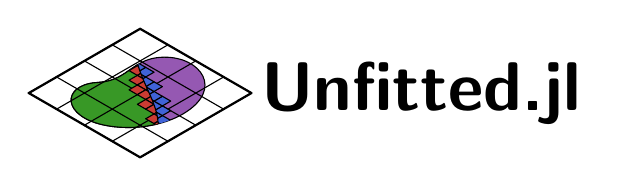
\begin{tikzpicture}[isometric view, rounded corners = 0.01mm]%
    \begin{scope}[canvas is xy plane at z = 0]
      % \fill[juliapurple] (-1cm, -1cm) rectangle (1cm, 1cm);
      \draw[\ink, thick] (-1cm, -1cm) rectangle (1cm, 1cm);


      \draw[\ink, fill = juliapurple] (-0.75, -0.3) to[closed, curve through = {(0.2, -0.7) (0.7, 0.4) (-0.15, 0.5)}] (-0.3, 0.6);
      
      \begin{scope}
        \clip (-1, -1) to[out = 10, in = 210] (1, 1) -- (-1, 1) -- cycle;
      
        \draw[\ink, fill = juliagreen] (-0.75, -0.3) to[closed, curve through = {(0.2, -0.7) (0.7, 0.4) (-0.15, 0.5)}] (-0.3, 0.6);
      \end{scope}

      \draw[\ink] (-1cm, -1cm) grid[step = 0.5cm] (1cm, 1cm);

      \begin{scope}
        \clip (-1, -1) to[out = 10, in = 210] (1, 1) -- (-1, 1) -- cycle;
        \clip (-0.75, -0.3) to[closed, curve through = {(0.2, -0.7) (0.7, 0.4) (-0.15, 0.5)}] (-0.3, 0.6);

        \draw[\ink, fill = juliared] (0.25cm, 0.3cm) rectangle ++(0.15cm, 0.15cm);
        \draw[\ink, fill = juliared] (0.25cm, 0.15cm) rectangle ++(0.15cm, 0.15cm);
        \draw[\ink, fill = juliared] (0.1cm, 0.15cm) rectangle ++(0.15cm, 0.15cm);
        \draw[\ink, fill = juliared] (0.1cm, 0cm) rectangle ++(0.15cm, 0.15cm);
        \draw[\ink, fill = juliared] (0.1cm, -0.15cm) rectangle ++(0.15cm, 0.15cm);
        \draw[\ink, fill = juliared] (-0.05cm, 0cm) rectangle ++(0.15cm, 0.15cm);
        \draw[\ink, fill = juliared] (-0.05cm, -0.15cm) rectangle ++(0.15cm, 0.15cm);
        \draw[\ink, fill = juliared] (-0.05cm, -0.3cm) rectangle ++(0.15cm, 0.15cm);
        \draw[\ink, fill = juliared] (-0.2cm, -0.3cm) rectangle ++(0.15cm, 0.15cm);
        \draw[\ink, fill = juliared] (-0.2cm, -0.45cm) rectangle ++(0.15cm, 0.15cm);
        \draw[\ink, fill = juliared] (-0.2cm, -0.6cm) rectangle ++(0.15cm, 0.15cm);
        \draw[\ink, fill = juliared] (-0.35cm, -0.6cm) rectangle ++(0.15cm, 0.15cm);
        \draw[\ink, fill = juliared] (-0.35cm, -0.75cm) rectangle ++(0.15cm, 0.15cm);
      \end{scope}

      \begin{scope}
        \clip (-1, -1) to[out = 10, in = 210] (1, 1) -- (1, -1) -- cycle;
        \clip (-0.75, -0.3) to[closed, curve through = {(0.2, -0.7) (0.7, 0.4) (-0.15, 0.5)}] (-0.3, 0.6);

        \draw[\ink, fill = juliablue] (-0.3cm, -0.7cm) rectangle ++(0.15cm, 0.15cm);
        \draw[\ink, fill = juliablue] (-0.3cm, -0.55cm) rectangle ++(0.15cm, 0.15cm);
        \draw[\ink, fill = juliablue] (-0.15cm, -0.55cm) rectangle ++(0.15cm, 0.15cm);
        \draw[\ink, fill = juliablue] (-0.15cm, -0.4cm) rectangle ++(0.15cm, 0.15cm);
        \draw[\ink, fill = juliablue] (-0cm, -0.4cm) rectangle ++(0.15cm, 0.15cm);
        \draw[\ink, fill = juliablue] (-0cm, -0.25cm) rectangle ++(0.15cm, 0.15cm);
        \draw[\ink, fill = juliablue] (-0cm, -0.1cm) rectangle ++(0.15cm, 0.15cm);
        \draw[\ink, fill = juliablue] (0.15cm, -0.1cm) rectangle ++(0.15cm, 0.15cm);
        \draw[\ink, fill = juliablue] (0.15cm, 0.05cm) rectangle ++(0.15cm, 0.15cm);
        \draw[\ink, fill = juliablue] (0.15cm, 0.2cm) rectangle ++(0.15cm, 0.15cm);
        \draw[\ink, fill = juliablue] (0.3cm, 0.2cm) rectangle ++(0.15cm, 0.15cm);
        \draw[\ink, fill = juliablue] (0.3cm, 0.35cm) rectangle ++(0.15cm, 0.15cm);
      \end{scope}

      \begin{scope}
        \clip (-0.75, -0.3) to[closed, curve through = {(0.2, -0.7) (0.7, 0.4) (-0.15, 0.5)}] (-0.3, 0.6);
        \draw[\ink] (-1, -1) to[out = 10, in = 210] (1, 1);
      \end{scope}

      \node[right, text = \ink] at (1, -1) {\Huge\sffamily\bfseries Unfitted.jl};
    \end{scope}
  \end{tikzpicture}%
\end{document}
'
%   dvisvgm --no-fonts --exact-bbox --bbox=1mm logo.dvi
%   dvisvgm --no-fonts --exact-bbox --bbox=1mm logo-dark.dvi
\providecommand{\ink}{black}

\begin{document}
  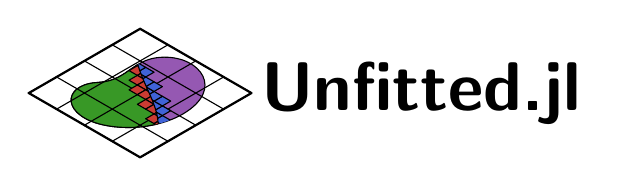
\begin{tikzpicture}[isometric view, rounded corners = 0.01mm]%
    \begin{scope}[canvas is xy plane at z = 0]
      % \fill[juliapurple] (-1cm, -1cm) rectangle (1cm, 1cm);
      \draw[\ink, thick] (-1cm, -1cm) rectangle (1cm, 1cm);


      \draw[\ink, fill = juliapurple] (-0.75, -0.3) to[closed, curve through = {(0.2, -0.7) (0.7, 0.4) (-0.15, 0.5)}] (-0.3, 0.6);
      
      \begin{scope}
        \clip (-1, -1) to[out = 10, in = 210] (1, 1) -- (-1, 1) -- cycle;
      
        \draw[\ink, fill = juliagreen] (-0.75, -0.3) to[closed, curve through = {(0.2, -0.7) (0.7, 0.4) (-0.15, 0.5)}] (-0.3, 0.6);
      \end{scope}

      \draw[\ink] (-1cm, -1cm) grid[step = 0.5cm] (1cm, 1cm);

      \begin{scope}
        \clip (-1, -1) to[out = 10, in = 210] (1, 1) -- (-1, 1) -- cycle;
        \clip (-0.75, -0.3) to[closed, curve through = {(0.2, -0.7) (0.7, 0.4) (-0.15, 0.5)}] (-0.3, 0.6);

        \draw[\ink, fill = juliared] (0.25cm, 0.3cm) rectangle ++(0.15cm, 0.15cm);
        \draw[\ink, fill = juliared] (0.25cm, 0.15cm) rectangle ++(0.15cm, 0.15cm);
        \draw[\ink, fill = juliared] (0.1cm, 0.15cm) rectangle ++(0.15cm, 0.15cm);
        \draw[\ink, fill = juliared] (0.1cm, 0cm) rectangle ++(0.15cm, 0.15cm);
        \draw[\ink, fill = juliared] (0.1cm, -0.15cm) rectangle ++(0.15cm, 0.15cm);
        \draw[\ink, fill = juliared] (-0.05cm, 0cm) rectangle ++(0.15cm, 0.15cm);
        \draw[\ink, fill = juliared] (-0.05cm, -0.15cm) rectangle ++(0.15cm, 0.15cm);
        \draw[\ink, fill = juliared] (-0.05cm, -0.3cm) rectangle ++(0.15cm, 0.15cm);
        \draw[\ink, fill = juliared] (-0.2cm, -0.3cm) rectangle ++(0.15cm, 0.15cm);
        \draw[\ink, fill = juliared] (-0.2cm, -0.45cm) rectangle ++(0.15cm, 0.15cm);
        \draw[\ink, fill = juliared] (-0.2cm, -0.6cm) rectangle ++(0.15cm, 0.15cm);
        \draw[\ink, fill = juliared] (-0.35cm, -0.6cm) rectangle ++(0.15cm, 0.15cm);
        \draw[\ink, fill = juliared] (-0.35cm, -0.75cm) rectangle ++(0.15cm, 0.15cm);
      \end{scope}

      \begin{scope}
        \clip (-1, -1) to[out = 10, in = 210] (1, 1) -- (1, -1) -- cycle;
        \clip (-0.75, -0.3) to[closed, curve through = {(0.2, -0.7) (0.7, 0.4) (-0.15, 0.5)}] (-0.3, 0.6);

        \draw[\ink, fill = juliablue] (-0.3cm, -0.7cm) rectangle ++(0.15cm, 0.15cm);
        \draw[\ink, fill = juliablue] (-0.3cm, -0.55cm) rectangle ++(0.15cm, 0.15cm);
        \draw[\ink, fill = juliablue] (-0.15cm, -0.55cm) rectangle ++(0.15cm, 0.15cm);
        \draw[\ink, fill = juliablue] (-0.15cm, -0.4cm) rectangle ++(0.15cm, 0.15cm);
        \draw[\ink, fill = juliablue] (-0cm, -0.4cm) rectangle ++(0.15cm, 0.15cm);
        \draw[\ink, fill = juliablue] (-0cm, -0.25cm) rectangle ++(0.15cm, 0.15cm);
        \draw[\ink, fill = juliablue] (-0cm, -0.1cm) rectangle ++(0.15cm, 0.15cm);
        \draw[\ink, fill = juliablue] (0.15cm, -0.1cm) rectangle ++(0.15cm, 0.15cm);
        \draw[\ink, fill = juliablue] (0.15cm, 0.05cm) rectangle ++(0.15cm, 0.15cm);
        \draw[\ink, fill = juliablue] (0.15cm, 0.2cm) rectangle ++(0.15cm, 0.15cm);
        \draw[\ink, fill = juliablue] (0.3cm, 0.2cm) rectangle ++(0.15cm, 0.15cm);
        \draw[\ink, fill = juliablue] (0.3cm, 0.35cm) rectangle ++(0.15cm, 0.15cm);
      \end{scope}

      \begin{scope}
        \clip (-0.75, -0.3) to[closed, curve through = {(0.2, -0.7) (0.7, 0.4) (-0.15, 0.5)}] (-0.3, 0.6);
        \draw[\ink] (-1, -1) to[out = 10, in = 210] (1, 1);
      \end{scope}

      \node[right, text = \ink] at (1, -1) {\Huge\sffamily\bfseries Unfitted.jl};
    \end{scope}
  \end{tikzpicture}%
\end{document}
'
%   latex -jobname=logo-dark '\def\pgfsysdriver{pgfsys-dvisvgm.def}\def\ink{white}\documentclass[margin = 1mm]{standalone}

\usepackage{tikz}
\usepackage[condensed]{roboto}

\usetikzlibrary{3d}
\usetikzlibrary{perspective}
\usetikzlibrary{hobby}

\definecolor{juliablue}{HTML}{4063D8}
\definecolor{juliagreen}{HTML}{389826}
\definecolor{juliared}{HTML}{CB3C33}
\definecolor{juliapurple}{HTML}{9558B2}

% Ink for every stroke in the drawing: the background mesh, the domain
% outline, the cell edges, the material interface and the wordmark. Fills stay
% fixed -- the four Julia colours read on either ground -- so the light and the
% dark asset differ in exactly one macro, and the dark variant is this same
% file compiled with `\ink' predefined.
%
% The README assets are SVG, built through DVI rather than PDF: dvisvgm only
% accepts PDF input via Ghostscript < 10.01 or mutool, while its DVI path is
% native and needs neither. `--no-fonts' traces the Roboto glyphs into paths
% so the wordmark does not depend on the font being installed, and `--bbox'
% restores the 1 mm margin that `--exact-bbox' would otherwise trim away.
%
%   latex -jobname=logo      '\def\pgfsysdriver{pgfsys-dvisvgm.def}\documentclass[margin = 1mm]{standalone}

\usepackage{tikz}
\usepackage[condensed]{roboto}

\usetikzlibrary{3d}
\usetikzlibrary{perspective}
\usetikzlibrary{hobby}

\definecolor{juliablue}{HTML}{4063D8}
\definecolor{juliagreen}{HTML}{389826}
\definecolor{juliared}{HTML}{CB3C33}
\definecolor{juliapurple}{HTML}{9558B2}

% Ink for every stroke in the drawing: the background mesh, the domain
% outline, the cell edges, the material interface and the wordmark. Fills stay
% fixed -- the four Julia colours read on either ground -- so the light and the
% dark asset differ in exactly one macro, and the dark variant is this same
% file compiled with `\ink' predefined.
%
% The README assets are SVG, built through DVI rather than PDF: dvisvgm only
% accepts PDF input via Ghostscript < 10.01 or mutool, while its DVI path is
% native and needs neither. `--no-fonts' traces the Roboto glyphs into paths
% so the wordmark does not depend on the font being installed, and `--bbox'
% restores the 1 mm margin that `--exact-bbox' would otherwise trim away.
%
%   latex -jobname=logo      '\def\pgfsysdriver{pgfsys-dvisvgm.def}\input{logo.tex}'
%   latex -jobname=logo-dark '\def\pgfsysdriver{pgfsys-dvisvgm.def}\def\ink{white}\input{logo.tex}'
%   dvisvgm --no-fonts --exact-bbox --bbox=1mm logo.dvi
%   dvisvgm --no-fonts --exact-bbox --bbox=1mm logo-dark.dvi
\providecommand{\ink}{black}

\begin{document}
  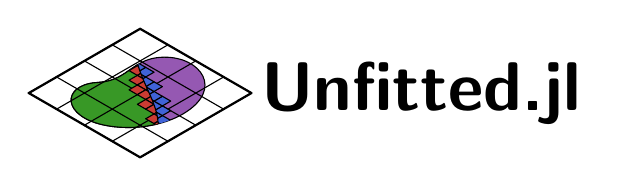
\begin{tikzpicture}[isometric view, rounded corners = 0.01mm]%
    \begin{scope}[canvas is xy plane at z = 0]
      % \fill[juliapurple] (-1cm, -1cm) rectangle (1cm, 1cm);
      \draw[\ink, thick] (-1cm, -1cm) rectangle (1cm, 1cm);


      \draw[\ink, fill = juliapurple] (-0.75, -0.3) to[closed, curve through = {(0.2, -0.7) (0.7, 0.4) (-0.15, 0.5)}] (-0.3, 0.6);
      
      \begin{scope}
        \clip (-1, -1) to[out = 10, in = 210] (1, 1) -- (-1, 1) -- cycle;
      
        \draw[\ink, fill = juliagreen] (-0.75, -0.3) to[closed, curve through = {(0.2, -0.7) (0.7, 0.4) (-0.15, 0.5)}] (-0.3, 0.6);
      \end{scope}

      \draw[\ink] (-1cm, -1cm) grid[step = 0.5cm] (1cm, 1cm);

      \begin{scope}
        \clip (-1, -1) to[out = 10, in = 210] (1, 1) -- (-1, 1) -- cycle;
        \clip (-0.75, -0.3) to[closed, curve through = {(0.2, -0.7) (0.7, 0.4) (-0.15, 0.5)}] (-0.3, 0.6);

        \draw[\ink, fill = juliared] (0.25cm, 0.3cm) rectangle ++(0.15cm, 0.15cm);
        \draw[\ink, fill = juliared] (0.25cm, 0.15cm) rectangle ++(0.15cm, 0.15cm);
        \draw[\ink, fill = juliared] (0.1cm, 0.15cm) rectangle ++(0.15cm, 0.15cm);
        \draw[\ink, fill = juliared] (0.1cm, 0cm) rectangle ++(0.15cm, 0.15cm);
        \draw[\ink, fill = juliared] (0.1cm, -0.15cm) rectangle ++(0.15cm, 0.15cm);
        \draw[\ink, fill = juliared] (-0.05cm, 0cm) rectangle ++(0.15cm, 0.15cm);
        \draw[\ink, fill = juliared] (-0.05cm, -0.15cm) rectangle ++(0.15cm, 0.15cm);
        \draw[\ink, fill = juliared] (-0.05cm, -0.3cm) rectangle ++(0.15cm, 0.15cm);
        \draw[\ink, fill = juliared] (-0.2cm, -0.3cm) rectangle ++(0.15cm, 0.15cm);
        \draw[\ink, fill = juliared] (-0.2cm, -0.45cm) rectangle ++(0.15cm, 0.15cm);
        \draw[\ink, fill = juliared] (-0.2cm, -0.6cm) rectangle ++(0.15cm, 0.15cm);
        \draw[\ink, fill = juliared] (-0.35cm, -0.6cm) rectangle ++(0.15cm, 0.15cm);
        \draw[\ink, fill = juliared] (-0.35cm, -0.75cm) rectangle ++(0.15cm, 0.15cm);
      \end{scope}

      \begin{scope}
        \clip (-1, -1) to[out = 10, in = 210] (1, 1) -- (1, -1) -- cycle;
        \clip (-0.75, -0.3) to[closed, curve through = {(0.2, -0.7) (0.7, 0.4) (-0.15, 0.5)}] (-0.3, 0.6);

        \draw[\ink, fill = juliablue] (-0.3cm, -0.7cm) rectangle ++(0.15cm, 0.15cm);
        \draw[\ink, fill = juliablue] (-0.3cm, -0.55cm) rectangle ++(0.15cm, 0.15cm);
        \draw[\ink, fill = juliablue] (-0.15cm, -0.55cm) rectangle ++(0.15cm, 0.15cm);
        \draw[\ink, fill = juliablue] (-0.15cm, -0.4cm) rectangle ++(0.15cm, 0.15cm);
        \draw[\ink, fill = juliablue] (-0cm, -0.4cm) rectangle ++(0.15cm, 0.15cm);
        \draw[\ink, fill = juliablue] (-0cm, -0.25cm) rectangle ++(0.15cm, 0.15cm);
        \draw[\ink, fill = juliablue] (-0cm, -0.1cm) rectangle ++(0.15cm, 0.15cm);
        \draw[\ink, fill = juliablue] (0.15cm, -0.1cm) rectangle ++(0.15cm, 0.15cm);
        \draw[\ink, fill = juliablue] (0.15cm, 0.05cm) rectangle ++(0.15cm, 0.15cm);
        \draw[\ink, fill = juliablue] (0.15cm, 0.2cm) rectangle ++(0.15cm, 0.15cm);
        \draw[\ink, fill = juliablue] (0.3cm, 0.2cm) rectangle ++(0.15cm, 0.15cm);
        \draw[\ink, fill = juliablue] (0.3cm, 0.35cm) rectangle ++(0.15cm, 0.15cm);
      \end{scope}

      \begin{scope}
        \clip (-0.75, -0.3) to[closed, curve through = {(0.2, -0.7) (0.7, 0.4) (-0.15, 0.5)}] (-0.3, 0.6);
        \draw[\ink] (-1, -1) to[out = 10, in = 210] (1, 1);
      \end{scope}

      \node[right, text = \ink] at (1, -1) {\Huge\sffamily\bfseries Unfitted.jl};
    \end{scope}
  \end{tikzpicture}%
\end{document}
'
%   latex -jobname=logo-dark '\def\pgfsysdriver{pgfsys-dvisvgm.def}\def\ink{white}\documentclass[margin = 1mm]{standalone}

\usepackage{tikz}
\usepackage[condensed]{roboto}

\usetikzlibrary{3d}
\usetikzlibrary{perspective}
\usetikzlibrary{hobby}

\definecolor{juliablue}{HTML}{4063D8}
\definecolor{juliagreen}{HTML}{389826}
\definecolor{juliared}{HTML}{CB3C33}
\definecolor{juliapurple}{HTML}{9558B2}

% Ink for every stroke in the drawing: the background mesh, the domain
% outline, the cell edges, the material interface and the wordmark. Fills stay
% fixed -- the four Julia colours read on either ground -- so the light and the
% dark asset differ in exactly one macro, and the dark variant is this same
% file compiled with `\ink' predefined.
%
% The README assets are SVG, built through DVI rather than PDF: dvisvgm only
% accepts PDF input via Ghostscript < 10.01 or mutool, while its DVI path is
% native and needs neither. `--no-fonts' traces the Roboto glyphs into paths
% so the wordmark does not depend on the font being installed, and `--bbox'
% restores the 1 mm margin that `--exact-bbox' would otherwise trim away.
%
%   latex -jobname=logo      '\def\pgfsysdriver{pgfsys-dvisvgm.def}\input{logo.tex}'
%   latex -jobname=logo-dark '\def\pgfsysdriver{pgfsys-dvisvgm.def}\def\ink{white}\input{logo.tex}'
%   dvisvgm --no-fonts --exact-bbox --bbox=1mm logo.dvi
%   dvisvgm --no-fonts --exact-bbox --bbox=1mm logo-dark.dvi
\providecommand{\ink}{black}

\begin{document}
  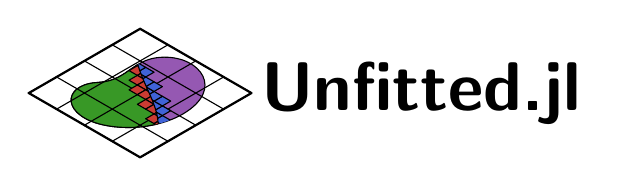
\begin{tikzpicture}[isometric view, rounded corners = 0.01mm]%
    \begin{scope}[canvas is xy plane at z = 0]
      % \fill[juliapurple] (-1cm, -1cm) rectangle (1cm, 1cm);
      \draw[\ink, thick] (-1cm, -1cm) rectangle (1cm, 1cm);


      \draw[\ink, fill = juliapurple] (-0.75, -0.3) to[closed, curve through = {(0.2, -0.7) (0.7, 0.4) (-0.15, 0.5)}] (-0.3, 0.6);
      
      \begin{scope}
        \clip (-1, -1) to[out = 10, in = 210] (1, 1) -- (-1, 1) -- cycle;
      
        \draw[\ink, fill = juliagreen] (-0.75, -0.3) to[closed, curve through = {(0.2, -0.7) (0.7, 0.4) (-0.15, 0.5)}] (-0.3, 0.6);
      \end{scope}

      \draw[\ink] (-1cm, -1cm) grid[step = 0.5cm] (1cm, 1cm);

      \begin{scope}
        \clip (-1, -1) to[out = 10, in = 210] (1, 1) -- (-1, 1) -- cycle;
        \clip (-0.75, -0.3) to[closed, curve through = {(0.2, -0.7) (0.7, 0.4) (-0.15, 0.5)}] (-0.3, 0.6);

        \draw[\ink, fill = juliared] (0.25cm, 0.3cm) rectangle ++(0.15cm, 0.15cm);
        \draw[\ink, fill = juliared] (0.25cm, 0.15cm) rectangle ++(0.15cm, 0.15cm);
        \draw[\ink, fill = juliared] (0.1cm, 0.15cm) rectangle ++(0.15cm, 0.15cm);
        \draw[\ink, fill = juliared] (0.1cm, 0cm) rectangle ++(0.15cm, 0.15cm);
        \draw[\ink, fill = juliared] (0.1cm, -0.15cm) rectangle ++(0.15cm, 0.15cm);
        \draw[\ink, fill = juliared] (-0.05cm, 0cm) rectangle ++(0.15cm, 0.15cm);
        \draw[\ink, fill = juliared] (-0.05cm, -0.15cm) rectangle ++(0.15cm, 0.15cm);
        \draw[\ink, fill = juliared] (-0.05cm, -0.3cm) rectangle ++(0.15cm, 0.15cm);
        \draw[\ink, fill = juliared] (-0.2cm, -0.3cm) rectangle ++(0.15cm, 0.15cm);
        \draw[\ink, fill = juliared] (-0.2cm, -0.45cm) rectangle ++(0.15cm, 0.15cm);
        \draw[\ink, fill = juliared] (-0.2cm, -0.6cm) rectangle ++(0.15cm, 0.15cm);
        \draw[\ink, fill = juliared] (-0.35cm, -0.6cm) rectangle ++(0.15cm, 0.15cm);
        \draw[\ink, fill = juliared] (-0.35cm, -0.75cm) rectangle ++(0.15cm, 0.15cm);
      \end{scope}

      \begin{scope}
        \clip (-1, -1) to[out = 10, in = 210] (1, 1) -- (1, -1) -- cycle;
        \clip (-0.75, -0.3) to[closed, curve through = {(0.2, -0.7) (0.7, 0.4) (-0.15, 0.5)}] (-0.3, 0.6);

        \draw[\ink, fill = juliablue] (-0.3cm, -0.7cm) rectangle ++(0.15cm, 0.15cm);
        \draw[\ink, fill = juliablue] (-0.3cm, -0.55cm) rectangle ++(0.15cm, 0.15cm);
        \draw[\ink, fill = juliablue] (-0.15cm, -0.55cm) rectangle ++(0.15cm, 0.15cm);
        \draw[\ink, fill = juliablue] (-0.15cm, -0.4cm) rectangle ++(0.15cm, 0.15cm);
        \draw[\ink, fill = juliablue] (-0cm, -0.4cm) rectangle ++(0.15cm, 0.15cm);
        \draw[\ink, fill = juliablue] (-0cm, -0.25cm) rectangle ++(0.15cm, 0.15cm);
        \draw[\ink, fill = juliablue] (-0cm, -0.1cm) rectangle ++(0.15cm, 0.15cm);
        \draw[\ink, fill = juliablue] (0.15cm, -0.1cm) rectangle ++(0.15cm, 0.15cm);
        \draw[\ink, fill = juliablue] (0.15cm, 0.05cm) rectangle ++(0.15cm, 0.15cm);
        \draw[\ink, fill = juliablue] (0.15cm, 0.2cm) rectangle ++(0.15cm, 0.15cm);
        \draw[\ink, fill = juliablue] (0.3cm, 0.2cm) rectangle ++(0.15cm, 0.15cm);
        \draw[\ink, fill = juliablue] (0.3cm, 0.35cm) rectangle ++(0.15cm, 0.15cm);
      \end{scope}

      \begin{scope}
        \clip (-0.75, -0.3) to[closed, curve through = {(0.2, -0.7) (0.7, 0.4) (-0.15, 0.5)}] (-0.3, 0.6);
        \draw[\ink] (-1, -1) to[out = 10, in = 210] (1, 1);
      \end{scope}

      \node[right, text = \ink] at (1, -1) {\Huge\sffamily\bfseries Unfitted.jl};
    \end{scope}
  \end{tikzpicture}%
\end{document}
'
%   dvisvgm --no-fonts --exact-bbox --bbox=1mm logo.dvi
%   dvisvgm --no-fonts --exact-bbox --bbox=1mm logo-dark.dvi
\providecommand{\ink}{black}

\begin{document}
  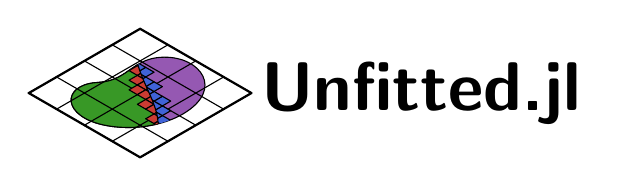
\begin{tikzpicture}[isometric view, rounded corners = 0.01mm]%
    \begin{scope}[canvas is xy plane at z = 0]
      % \fill[juliapurple] (-1cm, -1cm) rectangle (1cm, 1cm);
      \draw[\ink, thick] (-1cm, -1cm) rectangle (1cm, 1cm);


      \draw[\ink, fill = juliapurple] (-0.75, -0.3) to[closed, curve through = {(0.2, -0.7) (0.7, 0.4) (-0.15, 0.5)}] (-0.3, 0.6);
      
      \begin{scope}
        \clip (-1, -1) to[out = 10, in = 210] (1, 1) -- (-1, 1) -- cycle;
      
        \draw[\ink, fill = juliagreen] (-0.75, -0.3) to[closed, curve through = {(0.2, -0.7) (0.7, 0.4) (-0.15, 0.5)}] (-0.3, 0.6);
      \end{scope}

      \draw[\ink] (-1cm, -1cm) grid[step = 0.5cm] (1cm, 1cm);

      \begin{scope}
        \clip (-1, -1) to[out = 10, in = 210] (1, 1) -- (-1, 1) -- cycle;
        \clip (-0.75, -0.3) to[closed, curve through = {(0.2, -0.7) (0.7, 0.4) (-0.15, 0.5)}] (-0.3, 0.6);

        \draw[\ink, fill = juliared] (0.25cm, 0.3cm) rectangle ++(0.15cm, 0.15cm);
        \draw[\ink, fill = juliared] (0.25cm, 0.15cm) rectangle ++(0.15cm, 0.15cm);
        \draw[\ink, fill = juliared] (0.1cm, 0.15cm) rectangle ++(0.15cm, 0.15cm);
        \draw[\ink, fill = juliared] (0.1cm, 0cm) rectangle ++(0.15cm, 0.15cm);
        \draw[\ink, fill = juliared] (0.1cm, -0.15cm) rectangle ++(0.15cm, 0.15cm);
        \draw[\ink, fill = juliared] (-0.05cm, 0cm) rectangle ++(0.15cm, 0.15cm);
        \draw[\ink, fill = juliared] (-0.05cm, -0.15cm) rectangle ++(0.15cm, 0.15cm);
        \draw[\ink, fill = juliared] (-0.05cm, -0.3cm) rectangle ++(0.15cm, 0.15cm);
        \draw[\ink, fill = juliared] (-0.2cm, -0.3cm) rectangle ++(0.15cm, 0.15cm);
        \draw[\ink, fill = juliared] (-0.2cm, -0.45cm) rectangle ++(0.15cm, 0.15cm);
        \draw[\ink, fill = juliared] (-0.2cm, -0.6cm) rectangle ++(0.15cm, 0.15cm);
        \draw[\ink, fill = juliared] (-0.35cm, -0.6cm) rectangle ++(0.15cm, 0.15cm);
        \draw[\ink, fill = juliared] (-0.35cm, -0.75cm) rectangle ++(0.15cm, 0.15cm);
      \end{scope}

      \begin{scope}
        \clip (-1, -1) to[out = 10, in = 210] (1, 1) -- (1, -1) -- cycle;
        \clip (-0.75, -0.3) to[closed, curve through = {(0.2, -0.7) (0.7, 0.4) (-0.15, 0.5)}] (-0.3, 0.6);

        \draw[\ink, fill = juliablue] (-0.3cm, -0.7cm) rectangle ++(0.15cm, 0.15cm);
        \draw[\ink, fill = juliablue] (-0.3cm, -0.55cm) rectangle ++(0.15cm, 0.15cm);
        \draw[\ink, fill = juliablue] (-0.15cm, -0.55cm) rectangle ++(0.15cm, 0.15cm);
        \draw[\ink, fill = juliablue] (-0.15cm, -0.4cm) rectangle ++(0.15cm, 0.15cm);
        \draw[\ink, fill = juliablue] (-0cm, -0.4cm) rectangle ++(0.15cm, 0.15cm);
        \draw[\ink, fill = juliablue] (-0cm, -0.25cm) rectangle ++(0.15cm, 0.15cm);
        \draw[\ink, fill = juliablue] (-0cm, -0.1cm) rectangle ++(0.15cm, 0.15cm);
        \draw[\ink, fill = juliablue] (0.15cm, -0.1cm) rectangle ++(0.15cm, 0.15cm);
        \draw[\ink, fill = juliablue] (0.15cm, 0.05cm) rectangle ++(0.15cm, 0.15cm);
        \draw[\ink, fill = juliablue] (0.15cm, 0.2cm) rectangle ++(0.15cm, 0.15cm);
        \draw[\ink, fill = juliablue] (0.3cm, 0.2cm) rectangle ++(0.15cm, 0.15cm);
        \draw[\ink, fill = juliablue] (0.3cm, 0.35cm) rectangle ++(0.15cm, 0.15cm);
      \end{scope}

      \begin{scope}
        \clip (-0.75, -0.3) to[closed, curve through = {(0.2, -0.7) (0.7, 0.4) (-0.15, 0.5)}] (-0.3, 0.6);
        \draw[\ink] (-1, -1) to[out = 10, in = 210] (1, 1);
      \end{scope}

      \node[right, text = \ink] at (1, -1) {\Huge\sffamily\bfseries Unfitted.jl};
    \end{scope}
  \end{tikzpicture}%
\end{document}
'
%   dvisvgm --no-fonts --exact-bbox --bbox=1mm logo.dvi
%   dvisvgm --no-fonts --exact-bbox --bbox=1mm logo-dark.dvi
\providecommand{\ink}{black}

\begin{document}
  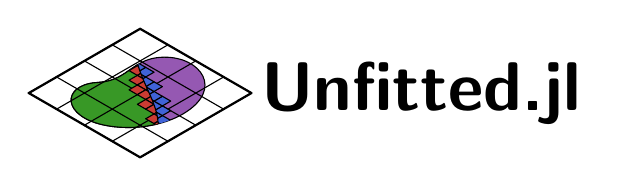
\begin{tikzpicture}[isometric view, rounded corners = 0.01mm]%
    \begin{scope}[canvas is xy plane at z = 0]
      % \fill[juliapurple] (-1cm, -1cm) rectangle (1cm, 1cm);
      \draw[\ink, thick] (-1cm, -1cm) rectangle (1cm, 1cm);


      \draw[\ink, fill = juliapurple] (-0.75, -0.3) to[closed, curve through = {(0.2, -0.7) (0.7, 0.4) (-0.15, 0.5)}] (-0.3, 0.6);
      
      \begin{scope}
        \clip (-1, -1) to[out = 10, in = 210] (1, 1) -- (-1, 1) -- cycle;
      
        \draw[\ink, fill = juliagreen] (-0.75, -0.3) to[closed, curve through = {(0.2, -0.7) (0.7, 0.4) (-0.15, 0.5)}] (-0.3, 0.6);
      \end{scope}

      \draw[\ink] (-1cm, -1cm) grid[step = 0.5cm] (1cm, 1cm);

      \begin{scope}
        \clip (-1, -1) to[out = 10, in = 210] (1, 1) -- (-1, 1) -- cycle;
        \clip (-0.75, -0.3) to[closed, curve through = {(0.2, -0.7) (0.7, 0.4) (-0.15, 0.5)}] (-0.3, 0.6);

        \draw[\ink, fill = juliared] (0.25cm, 0.3cm) rectangle ++(0.15cm, 0.15cm);
        \draw[\ink, fill = juliared] (0.25cm, 0.15cm) rectangle ++(0.15cm, 0.15cm);
        \draw[\ink, fill = juliared] (0.1cm, 0.15cm) rectangle ++(0.15cm, 0.15cm);
        \draw[\ink, fill = juliared] (0.1cm, 0cm) rectangle ++(0.15cm, 0.15cm);
        \draw[\ink, fill = juliared] (0.1cm, -0.15cm) rectangle ++(0.15cm, 0.15cm);
        \draw[\ink, fill = juliared] (-0.05cm, 0cm) rectangle ++(0.15cm, 0.15cm);
        \draw[\ink, fill = juliared] (-0.05cm, -0.15cm) rectangle ++(0.15cm, 0.15cm);
        \draw[\ink, fill = juliared] (-0.05cm, -0.3cm) rectangle ++(0.15cm, 0.15cm);
        \draw[\ink, fill = juliared] (-0.2cm, -0.3cm) rectangle ++(0.15cm, 0.15cm);
        \draw[\ink, fill = juliared] (-0.2cm, -0.45cm) rectangle ++(0.15cm, 0.15cm);
        \draw[\ink, fill = juliared] (-0.2cm, -0.6cm) rectangle ++(0.15cm, 0.15cm);
        \draw[\ink, fill = juliared] (-0.35cm, -0.6cm) rectangle ++(0.15cm, 0.15cm);
        \draw[\ink, fill = juliared] (-0.35cm, -0.75cm) rectangle ++(0.15cm, 0.15cm);
      \end{scope}

      \begin{scope}
        \clip (-1, -1) to[out = 10, in = 210] (1, 1) -- (1, -1) -- cycle;
        \clip (-0.75, -0.3) to[closed, curve through = {(0.2, -0.7) (0.7, 0.4) (-0.15, 0.5)}] (-0.3, 0.6);

        \draw[\ink, fill = juliablue] (-0.3cm, -0.7cm) rectangle ++(0.15cm, 0.15cm);
        \draw[\ink, fill = juliablue] (-0.3cm, -0.55cm) rectangle ++(0.15cm, 0.15cm);
        \draw[\ink, fill = juliablue] (-0.15cm, -0.55cm) rectangle ++(0.15cm, 0.15cm);
        \draw[\ink, fill = juliablue] (-0.15cm, -0.4cm) rectangle ++(0.15cm, 0.15cm);
        \draw[\ink, fill = juliablue] (-0cm, -0.4cm) rectangle ++(0.15cm, 0.15cm);
        \draw[\ink, fill = juliablue] (-0cm, -0.25cm) rectangle ++(0.15cm, 0.15cm);
        \draw[\ink, fill = juliablue] (-0cm, -0.1cm) rectangle ++(0.15cm, 0.15cm);
        \draw[\ink, fill = juliablue] (0.15cm, -0.1cm) rectangle ++(0.15cm, 0.15cm);
        \draw[\ink, fill = juliablue] (0.15cm, 0.05cm) rectangle ++(0.15cm, 0.15cm);
        \draw[\ink, fill = juliablue] (0.15cm, 0.2cm) rectangle ++(0.15cm, 0.15cm);
        \draw[\ink, fill = juliablue] (0.3cm, 0.2cm) rectangle ++(0.15cm, 0.15cm);
        \draw[\ink, fill = juliablue] (0.3cm, 0.35cm) rectangle ++(0.15cm, 0.15cm);
      \end{scope}

      \begin{scope}
        \clip (-0.75, -0.3) to[closed, curve through = {(0.2, -0.7) (0.7, 0.4) (-0.15, 0.5)}] (-0.3, 0.6);
        \draw[\ink] (-1, -1) to[out = 10, in = 210] (1, 1);
      \end{scope}

      \node[right, text = \ink] at (1, -1) {\Huge\sffamily\bfseries Unfitted.jl};
    \end{scope}
  \end{tikzpicture}%
\end{document}
'
%   dvisvgm --no-fonts --exact-bbox --bbox=1mm logo.dvi
%   dvisvgm --no-fonts --exact-bbox --bbox=1mm logo-dark.dvi
\providecommand{\ink}{black}

\begin{document}
  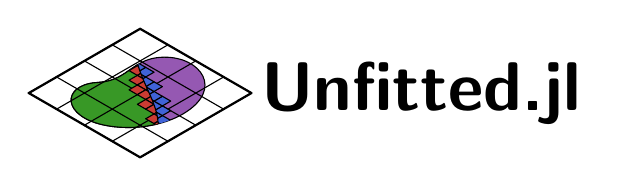
\begin{tikzpicture}[isometric view, rounded corners = 0.01mm]%
    \begin{scope}[canvas is xy plane at z = 0]
      % \fill[juliapurple] (-1cm, -1cm) rectangle (1cm, 1cm);
      \draw[\ink, thick] (-1cm, -1cm) rectangle (1cm, 1cm);


      \draw[\ink, fill = juliapurple] (-0.75, -0.3) to[closed, curve through = {(0.2, -0.7) (0.7, 0.4) (-0.15, 0.5)}] (-0.3, 0.6);
      
      \begin{scope}
        \clip (-1, -1) to[out = 10, in = 210] (1, 1) -- (-1, 1) -- cycle;
      
        \draw[\ink, fill = juliagreen] (-0.75, -0.3) to[closed, curve through = {(0.2, -0.7) (0.7, 0.4) (-0.15, 0.5)}] (-0.3, 0.6);
      \end{scope}

      \draw[\ink] (-1cm, -1cm) grid[step = 0.5cm] (1cm, 1cm);

      \begin{scope}
        \clip (-1, -1) to[out = 10, in = 210] (1, 1) -- (-1, 1) -- cycle;
        \clip (-0.75, -0.3) to[closed, curve through = {(0.2, -0.7) (0.7, 0.4) (-0.15, 0.5)}] (-0.3, 0.6);

        \draw[\ink, fill = juliared] (0.25cm, 0.3cm) rectangle ++(0.15cm, 0.15cm);
        \draw[\ink, fill = juliared] (0.25cm, 0.15cm) rectangle ++(0.15cm, 0.15cm);
        \draw[\ink, fill = juliared] (0.1cm, 0.15cm) rectangle ++(0.15cm, 0.15cm);
        \draw[\ink, fill = juliared] (0.1cm, 0cm) rectangle ++(0.15cm, 0.15cm);
        \draw[\ink, fill = juliared] (0.1cm, -0.15cm) rectangle ++(0.15cm, 0.15cm);
        \draw[\ink, fill = juliared] (-0.05cm, 0cm) rectangle ++(0.15cm, 0.15cm);
        \draw[\ink, fill = juliared] (-0.05cm, -0.15cm) rectangle ++(0.15cm, 0.15cm);
        \draw[\ink, fill = juliared] (-0.05cm, -0.3cm) rectangle ++(0.15cm, 0.15cm);
        \draw[\ink, fill = juliared] (-0.2cm, -0.3cm) rectangle ++(0.15cm, 0.15cm);
        \draw[\ink, fill = juliared] (-0.2cm, -0.45cm) rectangle ++(0.15cm, 0.15cm);
        \draw[\ink, fill = juliared] (-0.2cm, -0.6cm) rectangle ++(0.15cm, 0.15cm);
        \draw[\ink, fill = juliared] (-0.35cm, -0.6cm) rectangle ++(0.15cm, 0.15cm);
        \draw[\ink, fill = juliared] (-0.35cm, -0.75cm) rectangle ++(0.15cm, 0.15cm);
      \end{scope}

      \begin{scope}
        \clip (-1, -1) to[out = 10, in = 210] (1, 1) -- (1, -1) -- cycle;
        \clip (-0.75, -0.3) to[closed, curve through = {(0.2, -0.7) (0.7, 0.4) (-0.15, 0.5)}] (-0.3, 0.6);

        \draw[\ink, fill = juliablue] (-0.3cm, -0.7cm) rectangle ++(0.15cm, 0.15cm);
        \draw[\ink, fill = juliablue] (-0.3cm, -0.55cm) rectangle ++(0.15cm, 0.15cm);
        \draw[\ink, fill = juliablue] (-0.15cm, -0.55cm) rectangle ++(0.15cm, 0.15cm);
        \draw[\ink, fill = juliablue] (-0.15cm, -0.4cm) rectangle ++(0.15cm, 0.15cm);
        \draw[\ink, fill = juliablue] (-0cm, -0.4cm) rectangle ++(0.15cm, 0.15cm);
        \draw[\ink, fill = juliablue] (-0cm, -0.25cm) rectangle ++(0.15cm, 0.15cm);
        \draw[\ink, fill = juliablue] (-0cm, -0.1cm) rectangle ++(0.15cm, 0.15cm);
        \draw[\ink, fill = juliablue] (0.15cm, -0.1cm) rectangle ++(0.15cm, 0.15cm);
        \draw[\ink, fill = juliablue] (0.15cm, 0.05cm) rectangle ++(0.15cm, 0.15cm);
        \draw[\ink, fill = juliablue] (0.15cm, 0.2cm) rectangle ++(0.15cm, 0.15cm);
        \draw[\ink, fill = juliablue] (0.3cm, 0.2cm) rectangle ++(0.15cm, 0.15cm);
        \draw[\ink, fill = juliablue] (0.3cm, 0.35cm) rectangle ++(0.15cm, 0.15cm);
      \end{scope}

      \begin{scope}
        \clip (-0.75, -0.3) to[closed, curve through = {(0.2, -0.7) (0.7, 0.4) (-0.15, 0.5)}] (-0.3, 0.6);
        \draw[\ink] (-1, -1) to[out = 10, in = 210] (1, 1);
      \end{scope}

      \node[right, text = \ink] at (1, -1) {\Huge\sffamily\bfseries Unfitted.jl};
    \end{scope}
  \end{tikzpicture}%
\end{document}
